\documentclass[14pt, a4paper, oneside]{extarticle}

% Використання української мови
\usepackage[utf8]{inputenc}
\usepackage[T2A]{fontenc}
\usepackage[ukrainian]{babel}

\addto\captionsukrainian{\renewcommand{\refname}{ПЕРЕЛІК ДЖЕРЕЛ ПОСИЛАННЯ}}

\usepackage{titlesec}

\usepackage{tocloft}
\renewcommand{\cftsecleader}{\cftdotfill{\cftsecdotsep}}
\newlength{\mylen}
\settowidth{\mylen}{\cftsecpresnum}
\addtolength{\cftsecnumwidth}{\mylen}

\newcommand{\sectionbreak}{\clearpage}

% Задання розмірів полів
\usepackage{geometry}
\geometry{
  top=20mm,
  bottom=20mm,
  left=25mm,
  right=20mm
}

% Задання міжрядкового інтервалу 1.5
\usepackage{setspace}
\onehalfspacing

% Задання абзацного відступу 1.27 см
\usepackage{indentfirst}
\setlength{\parindent}{1.27cm}

\usepackage{setspace,amsmath}
\usepackage{tocloft}
\usepackage{indentfirst}
\usepackage{amsfonts}
\usepackage{wrapfig}
\usepackage{multicol}
\usepackage{lipsum}
\usepackage{lastpage}
\usepackage{listings}
\usepackage{titlesec}
\usepackage{tikz}

\usepackage{chngcntr}
\numberwithin{equation}{section}
\usepackage{graphicx}
\graphicspath{}
\DeclareGraphicsExtensions{.pdf,.png,.jpg}

\usepackage{graphicx}
\usepackage{caption}

% Налаштування підписів для рисунків
\captionsetup[figure]{
  labelsep = endash,  % Встановлює коротке тире після номера
  justification = centering,  % Центрування тексту підпису
  labelformat = simple,
  name = {Рисунок},  % Прибирає префікс "Рисунок"
}

% Налаштування формату "1.1 - Назва"
\renewcommand{\thefigure}{\arabic{section}.\arabic{figure}}


\usepackage{hyperref}
\hypersetup{
  colorlinks=false,
  linkcolor=blue,
  filecolor=magenta,      
  urlcolor=cyan,
  pdftitle={Applying the Generalization Principle to Solve Fuzzy Matrix Games}
}

\newcommand{\geqslant}{\geq}
\newcommand{\leqslant}{\leq}
\newcommand{\preccurlyeq}{\preceq}
\newcommand{\succcurlyeq}{\succeq}

\newcommand{\addition}{\section{ДОДАТОК}}

\usepackage{titlesec}

% Заголовки рівня \section
\titleformat{\section}
  {\normalfont\fontsize{14}{17}\bfseries\filcenter\MakeUppercase}
  {\thesection}
  {1em}
  {}

% Заголовки рівня \subsection
\titleformat{\subsection}
  {\normalfont\fontsize{14}{17}\bfseries}
  {\thesubsection}
  {1em}
  {}

% Заголовки рівня \subsubsection
\titleformat{\subsubsection}
  {\normalfont\fontsize{14}{17}\bfseries}
  {\thesubsubsection}
  {1em}
  {}

% Відстань між заголовками та текстом
\titlespacing*{\section}{0pt}{3.25ex plus 1ex minus .2ex}{3ex}
\titlespacing*{\subsection}{0pt}{3.25ex plus 1ex minus .2ex}{3ex}
\titlespacing*{\subsubsection}{0pt}{3.25ex plus 1ex minus .2ex}{3ex}

% Задання стилю нумерації для основного тексту
\usepackage{fancyhdr}
\pagestyle{fancy}
\fancyhf{}
\fancyhead[R]{\thepage}
\renewcommand{\headrulewidth}{0pt}
\renewcommand{\footrulewidth}{0pt}

% Відключення нумерації на титульному аркуші
\pagenumbering{arabic}
\thispagestyle{empty}

\begin{document}

\begin{center}
\textbf{КИЇВСЬКИЙ НАЦІОНАЛЬНИЙ УНІВЕРСИТЕТ\\ ІМЕНІ ТАРАСА ШЕВЧЕНКА}\\ 
Факультет комп'ютерних наук та кібернетики\\
Кафедра системного аналізу та теорії прийняття рішень\\

\vfill

\textbf{\large{Кваліфікаційна робота}}\\
\textbf{на здобуття ступеня магістра}\\
за освітньо-науковою програмою <<Системи і методи прийняття рішень>>\\
за спеціальністю 124 Системний аналіз\\
на тему:\\
\textbf{МАТРИЧНА ГРА З НЕЧІТКИМИ МНОЖИНАМИ СТРАТЕГІЙ ГРАВЦІВ}

\vfill

\end{center}

\begin{flushleft}

Виконав студент 2-го курсу магістратури\\
Денис ПІВЕНЬ \hfill \underline{\hspace{3cm}}\\
\end{flushleft}

\begin{flushleft}
Науковий керівник:\\
професор, доктор фіз.-мат.наук.\\
Сергій МАЩЕНКО \hfill \underline{\hspace{3cm}}
\end{flushleft}

\vfill

\begin{multicols}{2}
  \hspace{1mm}

  \columnbreak
    Засвідчую, що в цій роботі немає запозичень з праць інших авторів без відповідних посилань.
    \\
    Студент \hfill \underline{\hspace{3cm}}

\hspace{1mm}

    Роботу розглянуто й допущено до захисту на засіданні кафедри системного аналізу та теорії прийняття рішень
    \\
    <<\underline{\hspace{1cm}}>> \underline{\hspace{3cm}} 2024р.,\\
    протокол №\underline{\hspace{1cm}}\\
    Завідувач кафедри\\
    Олена КАПУСТЯН \hfill \underline{\hspace{3cm}}
    
  
\end{multicols}

\vfill

\centerline{Київ – 2024}

\section*{Реферат}
Обсяг роботи 54 сторінки, 1 рисунок, 1 таблиця, 29 джерел посилань, 1 додаток. 

НЕЧІТКА МАТРИЧНА ГРА, НЕЧІТКІ МНОЖИНИ, НЕЧІТКІ МНОЖИНИ ТИПУ-2.

Матричні ігри з нечіткими стратегіями гравців займають важливе місце у прикладній математиці, теорії ігор та прийняття рішень. Ця область приваблює значну увагу фахівців, що шукають нові методи для аналізу складних систем, де взаємодії між агентами характеризуються невизначеністю та конфліктністю.

Об'єктом дослідження є матричні ігри із нечіткими множинами стратегій гравців.

Предметом дослідження є методи розв'язання матричних ігор з нечіткими множинами стратегій гравців.

Метою роботи є розробка, демонстрація на прикладах та програмна реалізація методу, який дозволить учасникам ігрового процесу знайти ціну гри в умовах нечіткості множин стратегій. 

Методи розроблення: теорія нечітких множин, теорія ігор, оптимізаційні методи. 

Інструменти розроблення: програмувальне середовище IntelliJ IDEA, мова програмування Java, фреймворк Spring Boot, платформа для управління контейнерами Docker. 

Результати роботи: проведено огляд з теорії нечітких множин, методів розв'язання нечітких матричних ігор; обґрунтовано те, що ціною гри з нечіткими множинами стратегій гравців є нечітка множина типу-2 спеціального виду; досліджені властивості цієї множини; розроблено декомпозиційний метод побудови нечіткої множина типу-2 ціни гри; здійснено програмну реалізацію розробленого методу.


\clearpage
\renewcommand\cftsecdotsep{\cftdot}
\cftsetpnumwidth{9pt}

% Задання форматування назви змісту
\renewcommand{\cfttoctitlefont}{\hfill\Large\bfseries\MakeUppercase}
\renewcommand{\cftaftertoctitle}{\hfill}

% Задання форматування для рівнів заголовків
\renewcommand{\cftsecfont}{\normalfont}
\renewcommand{\cftsecpagefont}{\normalfont}
\renewcommand{\cftsubsecfont}{\normalfont}
\renewcommand{\cftsubsecpagefont}{\normalfont}
\renewcommand{\cftsubsubsecfont}{\normalfont}
\renewcommand{\cftsubsubsecpagefont}{\normalfont}

% Задання відстані між рядками
\renewcommand{\cftbeforesecskip}{0.5ex}
\renewcommand{\cftbeforesubsecskip}{0.5ex}
\renewcommand{\cftbeforesubsubsecskip}{0.5ex}

\tableofcontents

\thispagestyle{empty}


\section*{СКОРОЧЕННЯ ТА УМОВНІ ПОЗНАЧЕННЯ}
\addcontentsline{toc}{section}{СКОРОЧЕННЯ ТА УМОВНІ ПОЗНАЧЕННЯ}

\begin{description}
    \item[НМ] -- Нечітка множина
    \item[НМТ-1] -- Нечітка множина типу-1
    \item[НМТ-2] -- Нечітка множина типу-2
    \item[ОПР] -- Особа приймаюча рішення
    \item[ТНЧ] -- Трикутне нечітке число
    \item[ФН] -- Функція належності
    \item[ФНТ-2] -- Функція належності типу-2
    \item[IDE] -- Integrated Development Environment
\end{description}


\section*{ВСТУП}
\addcontentsline{toc}{section}{ВСТУП}
У некооперативних іграх часто виникає ситуація, коли гравці не можуть чітко визначити свої стратегії та оцінити потенційні виграші через невизначеність людських суджень та неточності в аналізі реальних конфліктних ситуацій. В таких умовах теорія нечітких множин виявляється корисним інструментом для моделювання та розв'язання цих проблем.

Моделі з нечіткими множинами стратегій та нечіткими стратегіями або не використовують нечіткі оцінки результатів взагалі, або використовують їх опосередковано через нечіткі цілі за допомогою підходу Беллмана-Заде. Можливо, це є причиною їхньої обчислювальної складності та обмеженого застосування. Для спрощення вивчатимемо значення нечіткої матричної гри без зосередження на <<оптимальних>> стратегіях гравців. Також сенс такого дослідження може бути пояснений тим фактом, що ігрові задачі цікаві не тільки з погляду знаходження <<оптимальних>> стратегій гравців. Іноді значення гри має незалежний інтерес, оскільки область теорії ігор може включати прогнозування та аналіз конфліктних ситуацій як з думки гравців, так і деяких зовнішніх агентів. Метою такого аналізу може бути прийняття рішень, пов'язаних зі змінами у передумовах, умовах та наслідках конфлікту. Наприклад, це може бути зміна рівня інформованості, різні форми кооперативної взаємодії тощо. Формалізація стратегій у вигляді нечітких множин дозволяє врахувати у моделі гри не тільки невизначеність в оцінці гравцями допустимості вибору стратегій партнера, але й нечіткість у розумінні, які стратегії гравців прийнятні для вибору. Прикладами таких нечітких множин стратегій можуть бути: <<Перевірені стратегії>>, <<Стійкі стратегії>> тощо.

Особлива увага у роботі приділена розробці методу знаходження ціни гри в умовах використання для нечітких множин стратегій гравців. Був розроблений застосунок для знаходження ціни гри у змішаних стратегіях, який дозволяє застосовувати на практиці розроблений метод для різноманітних сценаріїв гри. Цей застосунок є інструментом для глибшого розуміння взаємодій між гравцями в умовах нечіткої інформації, що може зробити його корисним у теорії ігор.

\section{ОГЛЯД З ТЕОРІЇ ІГОР З НЕЧІТКИМИ ПАРАМЕТРАМИ}

Теорія ігор з нечіткими параметрами є узагальненням класичної теорії ігор, яке дозволяє враховувати в постановці гри нечіткість параметрів, що до неї входять, таких як виграш або стратегії гравців. Однією з основних ідей є використання теорії нечітких множин для представлення нечіткості параметрів гри. У зв'язку з цим, в теорії ігор з нечіткими параметрами застосовуються різні види нечітких множин, такі як трикутні нечіткі множини, трапецієподібні нечіткі множини та інші.

Основні поняття теорії ігор з нечіткими параметрами включають нечітку функцію виграшу, нечіткі множини стратегій гравців, виграшів та нечіткі оптимальні стратегії гравця. Теорія ігор з нечіткими параметрами має важливі застосування в різних галузях, таких як економіка, управління та прийняття рішень. Вона дозволяє аналізувати ігри в умовах невизначеності та недостатньої інформації.

\subsection{Нечіткі множини}

У традиційній прикладній математиці множина розуміється як сукупність елементів, що мають спільну властивість. Наприклад, множина чисел, що не менше заданого числа, множина векторів, сума компонент яких не перевищує одиницю та інше. При цьому для будь-якого елемента розглядаються лише дві можливості: або цей елемент належить до множини, або ні.

У теорії нечітких множин  допускається існування елементів, які можуть належати до множини з різним ступенем. Такі множини називаються нечіткими.

Поняття нечіткого множини є спробою математичної формалізації нечіткої інформації з метою її використання при побудові математичних моделей складних систем. В основі цього поняття лежить ідея того, що елементи, які складають дану множину і мають спільну властивість, можуть мати цю властивість в різній мірі, отже, належати до даної множини з різним ступенем. При такому підході висловлювання типу <<елемент $х$ належить даній множині>> втрачає зміст, оскільки потрібно вказати наскільки сильно або з яким ступенем даний елемент належить до даної множини.

Нечітка множина $C$ у множині $X$ визначається як сукупність пар виду $(x, \mu(x))$, де x належить $X$, а $\mu(x)$ є функцією, яка призначає ступінь належності елементу $x$ в $C$. Таким чином, нечітка множина є ширшим поняттям, ніж звичайна, в тому сенсі, що функція належності нечіткої множини може бути, взагалі будь-якою функцією або навіть довільним відображенням.

Нечітка множина називається \textit{порожньою}, якщо її функція належності дорівнює нулю на всій множині $X$, тобто
\begin{equation*}
    \mu_\emptyset (x) = 0, \forall x \in X,
\end{equation*}
Універсальну множину $X$ також можна описати функцією належності виду
\begin{equation*}
\mu_X (x) = 1, \forall x \in X,
\end{equation*}
\textit{Носієм} нечіткої множини $A$ (позначається $supp A$) з функцією належності $\mu_A (x)$ називається множина (у звичайному сенсі) виду
\begin{equation*}
\operatorname{supp} A=\left\{x \mid x \in X, \mu_A(x)>0\right\},
\end{equation*}
Нечітка множина $А$ називається \textit{нормальною}, якщо виконується рівність
\begin{equation*}
\sup _{x \in X} \mu_A(x)=1,
\end{equation*}
В іншому випадку нечітка множина називається \textit{субнормальною}.

Нехай $A$ та $B$ -- нечіткі множини в $X$, а $\mu_{A}(x)$ та $\mu_B(x)$ -- їхні функції належності відповідно. Кажуть, що $A$ \textit{містить у собі} $B$ (тобто $B \subseteq A$ ), якщо для будь-якого $x \in X$ виконується нерівність $\mu_B(x) \leq \mu_A(x)$. Множини $A$ та $B$ \textit{співпадають}, якщо $\mu_B(x)=\mu_A(x)$ при будь-якому $x \in X$. Якщо нечіткі множини $A$ та $B$ такі, що $B \subseteq A$, то
\begin{equation*}
\operatorname{supp} B \subseteq \operatorname{supp} A.\end{equation*}
\subsubsection{Операції над нечіткими множинами}
Операції над нечіткими множинами, наприклад, об'єднання та перетин, можна визначити різними способами. Нижче наведено декілька таких визначень. Вибір конкретного з них залежить від змісту, який вкладається в відповідну операцію в рамках задачі, що розглядається.

При введенні операцій над нечіткими множинами слід пам'ятати, що клас нечітких множин охоплює і множини у звичайному розумінні. Тому введення визначень в окремому випадку звичайних множин є необхідним у теорії множин. Звичайно, це не стосується до технічних питань, пов'язаних з операціями над нечіткими множинами які для звичайних множин не мають сенсу, наприклад, операції концентрування, розтягування та опуклої комбінації.

\textit{Операція об'єднання нечітких множин} $A$ та $B$ в $X$ визначається як нечітка множина $A \cup B$ з функцією належності вигляду:
\begin{equation*}
\mu_{A \cup B}(x)=\max \left\{\mu_A(x), \mu_B(x)\right\}, \quad x \in X,
\end{equation*}
Якщо $\{A_y\}$ -- скінчене або нескінчене сімейство нечітких множин з функціями належності $\mu_{A_y}(x, y)$, де $y \in Y$ -- параметр сімейства, то об'єднання $~C~=~\bigcup_Y A_y$ множин цього сімейства є нечіткою множиною з функцією належності вигляду
\begin{equation*}
\mu_C(x)=\sup _{y \in Y} \mu_{A_y}(x, y), \quad x \in X,
\end{equation*}
\textit{об'єднання нечітких множин} $A$ і $B$ в $X$ можна визначити за допомогою алгебраїчної суми їх функцій належності:
\begin{equation*}
\mu_{A \cup B}(x)=\left\{\begin{array}{cc}
1 & \text { при } \mu_A(x)+\mu_B(x) \geq 1, \\
\mu_A(x)+\mu_B(x) & \text { інакше. }
\end{array}\right.
\end{equation*}
Перетином нечітких множин $A$ та $B$ в $X$ називається нечітка множина $A \cap B$ з функцією належності виду
\begin{equation*}
\mu_{A \cap B}(x)=\min \left\{\mu_A(x), \mu_B(x)\right\}, \quad x \in X.
\end{equation*}
Якщо ${A_y}$ -- нескінчене чи скінчене сімейство нечітких множин з функціями належності $\mu_{A_y}(x, y)$, де $y \in Y$ -- параметр сімейства, то перетином $C~=~\bigcap_{y} A_y$ множин цього сімейства є нечітка множина з функцією належності виду
\begin{equation*}
\mu_C(x)=\inf _{y \in Y} \mu_{A_y}(x, y), \quad x \in X ,
\end{equation*}
Ще один спосіб визначення перетину нечітких множин $A$ та $B$ -- використання алгебраїчного добутку їх функцій належності:
\begin{equation*}
\mu_{A \cap B}(x)=\mu_A(x) \mu_B(x), \quad x \in X,
\end{equation*}
Майже всі відмінності між цими визначеннями проявляються у випадку нечітких множин $A$ та $B$, таких, що $B \subseteq A$, тобто $\mu_B(x) \subseteq \mu_A(x)$ для будь-якого $x \in X$. За першим з цих визначень
\begin{equation*}
\mu_{A \cap B}(x)=\mu_B(x), \quad x \in X,
\end{equation*}
тобто функція належності множини $A$ фактично не бере участь у цьому визначенні у відповідній функції належності, тоді як за визначенням добутку функція належності завжди містить функції належності обох множин.

Корисними можуть бути наступні властивості нечітких множин:
\begin{equation*}
\begin{aligned}
& \operatorname{supp}(A \cup B)=(\operatorname{supp} A) \cup(\operatorname{supp} B), \\
& \operatorname{supp}(A \cap B)=(\operatorname{supp} A) \cap(\operatorname{supp} B).
\end{aligned}
\end{equation*}
Легко перевірити, що ці рівності виконуються для будь-якого з наведених вище визначень об'єднання та перетину.

\textit{Доповненням нечіткої множини} $A$ в $X$ є нечітка множина $A^{\prime}$ з функцією належності, визначеною наступним чином:
\begin{equation*}
\mu_{A^{\prime}}(x)=1-\mu_A(x), \quad x \in X.
\end{equation*}
Цікаво, що з таким визначенням доповнення, взагалі кажучи, $A \cap A^{\prime} \neq \emptyset$ (це відрізняє його від стандартних множин).

\textit{Різницею нечітких множин} $A$ і $B$ в $X$ називається нечітка множина $A \backslash B$ з функцією належності виду
\begin{equation*}\mu_{A \backslash B}(x)=
\begin{cases}
\mu_A(x)-\mu_B(x) & \text { при } \mu_A(x) \geq \mu_B(x),\\
0 & \text { інакше. }
\end{cases}\end{equation*}
Зауважимо, що приведене вище визначення доповнення нечіткої множини випливає з даного визначення.

\textit{Декартовим добутком нечітких множин} $A_1, \ldots, A_n$ у $X_1, \ldots, X_n$, відповідно, називається нечітка множина $A$ у декартовому добутку $X=X_1 \times \ldots \times X_n$ з функцією належності виду:
\begin{equation*}
\begin{aligned}
\mu_A(x) & =\min \left\{\mu_{A_1}\left(x_1\right), \ldots, \mu_{A_n}\left(x_n\right)\right\}, \\
x & =\left(x_1, \ldots, x_n\right) \in X .
\end{aligned}
\end{equation*}
\textit{Опуклою комбінацією нечітких множин} $A_1, \ldots, A_n$ в $X$ називається нечітка множина $A$ з функцією належності вигляду:
\begin{equation*}
\begin{aligned}
& \mu_{A}(x)=\sum_{i=1}^n \lambda_i \mu_i(x), \\
& \text {де}, \lambda_i \geq 0, \quad i=1,2, \ldots, n, \quad\sum_{i=1}^n \lambda_i=1 .
\end{aligned}
\end{equation*}
Опуклі комбінації нечітких множин можуть застосовуватися, наприклад, у задачах прийняття рішень з кількома нечіткими обмеженнями. Зауважимо, що для звичайних множин ця операція не має сенсу.

\textit{Операції концентрування (CON) та розтягування (DIL) нечіткої множини} $A$ визначаються наступним чином:
\begin{align*}
& \operatorname{CON} A = A^2, \quad \operatorname{DIL} A = A^{0.5},\\
& \text{де } \mu_{A^\alpha}(x) = \mu_A^\alpha(x), \quad x\in X, \alpha > 0.
\end{align*}

Застосування операції концентрування до заданої нечіткої множини фактично означає зменшення <<нечіткості>> цієї множини. У реальній ситуації це може означати отримання нової інформації, що дозволяє більш точно (більш чітко) описати поняття нечіткої множини. Аналогічним чином, операцію розтягування можна застосовувати для моделювання ситуації, пов'язаної з втратою інформації.

\subsubsection{Множини рівня та декомпозиція нечіткої множини}

Множина рівня $\alpha$ нечіткої множини $A$ в $X$ називається множиною у звичайному розумінні, складеною з елементів $x \in X$, ступінь належності яких до нечіткої множини $A$ не менше числа $\alpha$. Таким чином, якщо $A_\alpha$ -- множина рівня $\alpha$ нечіткої множини $A$, то
\begin{equation*}
A_a=\left\{x \mid x \in X, \quad \mu_A(x) \geq \alpha\right\} .
\end{equation*}
Як буде показано нижче, множинами рівня зручно користуватися при формулюванні та аналізі деяких задач прийняття рішень.

Нехай $(A \cup B)_\alpha$ та $(A \cap B)_\alpha$ -- множини рівня $\alpha$ об'єднання та перетину нечітких множин $A$ та $B$ відповідно. Розглянемо зв'язок цих множин з множинами рівня $A_\alpha$ та $B_{\alpha}$. Якщо прийняти перші визначення об'єднання та перетину, то, як легко бачити, цей зв'язок такий:
\begin{equation*}
(A \cup B)_\alpha=A_\alpha \cup B_\alpha, \quad(A \cap B)_\alpha=A_\alpha \cap B_{\alpha}.
\end{equation*}
У випадку інших визначень маємо лише:
\begin{equation*}
(A \cup B)_\alpha \supset A_\alpha \cup B_\alpha, \quad(A \cap B)_\alpha \subset A_\alpha \cap B_{\alpha}.
\end{equation*}
Якщо $\left(A_1 \times \ldots \times A_n\right)_\alpha$ -- множина рівня $\alpha$ декартового добутку нечітких множин $A_1, \ldots, A_n$, то з визначення декартового добутку легко бачити, що
\begin{equation*}
\left(A_1 \times \ldots \times A_n\right)_\alpha=\left(A_1\right)_\alpha \times \ldots \times\left(A_n\right)_\alpha,
\end{equation*}
тобто множина рівня $\alpha$ декартового добутку є декартовим добутком множин рівня $\alpha$ його нечітких множин.

Множина $\left(A_\alpha\right)$ рівня $\alpha$ будь-якої опуклої комбінації нечітких множин $A_1, \ldots, A_n$ містить перетин множин рівня $\alpha$ усіх її множин, тобто
\begin{equation*}
\bigcap_{i=1}^n\left(A_i\right)_\alpha \subset A_{\alpha}.
\end{equation*}
В деяких випадках зручно використовувати розклад нечіткої множини за її множинам рівня, тобто представлення її у вигляді
\begin{equation*}
A=\bigcup_\alpha \alpha A_\alpha,
\end{equation*}
де $\mu_{\alpha A_\alpha}(x)=\alpha \mu_{A_\alpha}(x)$, а об'єднання нечітких множин $\alpha A_\alpha$ береться відповідно до визначення по всім $\alpha$ від 0 до 1.

\subsubsection{Нечіткі множини типу-2}
Нечіткі множини типу-2 (НМТ-2) є розширенням нечітких множин типу-1 (НМТ-1). НМТ-2, позначимо її через $\tilde{C}$, на чіткій множині $X$ характеризується нечіткою функцією належності $M_{\tilde{C}}: X \rightarrow[0,1]^{[0,1]}$. Для фіксованого $x^{\prime} \in X$ значення функції належності $M_{\tilde{C}}\left(x^{\prime}\right)$ називається нечітким ступенем належності. 

Воно представляє НМТ-1 $M_{\tilde{C}}\left(x^{\prime}\right)=\left\{\left(u, \mu_{M_{\tilde{C}}\left(x^{\prime}\right)}(u)\right): u \in J_{x^{\prime}}\right\}$ на множині $J_{x^{\prime}} \subseteq[0,1]$ первинних ступенів належності $u$ до $\tilde{C}$ з відповідною функцією належності $\mu_{M_{\tilde{C}}\left(x^{\prime}\right)}(u), u \in J_{x^{\prime}}$. НМТ-2 $\tilde{C}$ у вигляді
\begin{equation*}
\tilde{C}=\left\{\left(x, M_{\tilde{C}}(x)\right): x \in X\right\}=\left\{\left(x,\left\{\left(u, \mu_{M_{\tilde{C}}(x)}(u)\right): u \in U_{x}\right\}\right): x \in X\right\},
\end{equation*}
називається представленою у вертикальних зрізах.

Інше визначення, на основі ідей Карніка та Мендела \cite{Karnik}, було дано Менделем та Джоном \cite{Mendel}. НМТ-2 $\tilde{C}$ на чіткій множині $X$ характеризується функцією належності типу-2 (ФНТ-2) $\eta_{\tilde{C}}(x, u)$, тобто,
\begin{equation*}
\tilde{C}=\left\{\left((x, u), \eta_{\tilde{C}}(x, u)\right): x \in X, u \in[0,1]\right\},
\end{equation*}
де значення $\eta_{\tilde{C}}(x, u)$ є чітким числом з інтервалу $[0,1]$, відомим як вторинна оцінка пари $(x, u)$ до $\tilde{C}$. НМТ-2 $\tilde{C}$ з ФНТ-2 $\eta_{\tilde{C}}(x, u)$ завжди може бути представленою у вертикальних зрізах наступним чином
\begin{equation*}
\begin{aligned}
& \tilde{C}=\left\{\left((x, u), \eta_{\tilde{C}}(x, u)\right): x \in X, u \in[0,1]\right\}= \\
& \left\{\left(x,\left\{\left(u, \mu_{M_{\tilde{C}}(x)}(u)\right): u \in U_{x}\right\}\right): x \in X\right\}=\left\{\left(x, M_{\tilde{C}}(x)\right): x \in X\right\},
\end{aligned}
\end{equation*}
і навпаки. Тут множина первинних ступенів належності $U_{x} \subseteq[0,1]$ може розглядатися як носій нечіткого ступеня належності $M_{\tilde{C}}(x)$ до $\tilde{C}$, де $\mu_{M_{\tilde{C}}(x)}(u)=\eta_{\tilde{C}}(x, u), u \in U_{x}$. Тому, при розгляді ФНТ-2 $\eta_{\tilde{C}}(x, u)$ для всіх $u \in[0,1]$, припускається, що $\eta_{\tilde{C}}(x, u)=0$ для всіх $u \notin U_{x}$.

\textbf{Зауваження 1.1.} Первинний ступінь належності $u \in[0,1]$ зазвичай розуміється як ступінь прояву деякої властивості (яка визначає дану нечітку множину) для $x \in X$. Вторинна оцінка зазвичай асоціюється з оцінкою істинності відповідного первинного ступеня $u$ цієї властивості для $x$.

Визначаємо НМТ-2 та НМТ-1, вкладені в НМТ-2
\begin{equation*}
\tilde{C}=\left\{\left((x, u), \eta_{\tilde{C}}(x, u)\right): x \in X, u \in[0,1]\right\}.
\end{equation*}
Припустимо, що $u_{x}=\mu_{C^{e 1}}(x) \in[0,1]$ є єдиним первинним ступенем належності для кожного $x \in X$, де $\mu_{C^{e 1}}(x)$, $x \in X$ є функцією належності НМТ-1 $C^{e 1}=\left\{\left(x, \mu_{C^{e 1}}\right): x \in X\right\}$. Ця НМТ-1 називається вкладеною в НМТ-2 $\tilde{C}$. Визначаємо вкладену НМТ-2 $\tilde{C}^{e 2}$ у $\tilde{C}$ у вигляді \\$\tilde{C}^{e 2}=\left\{\left(\left(x, u_{x}\right), \eta_{\tilde{C}^{e 2}}\left(x, u_{x}\right)\right): x \in X\right\}$ з $\eta_{\tilde{C}^{e 2}}\left(x, u_{x}\right)=\eta_{\tilde{C}}\left(x, \mu_{C^{e 1}}(x)\right)$, $x \in X$.

\textbf{Зауваження 1.2.} Кожен елемент сукупності $\tilde{C}=\{\left((x, u), \eta_{\tilde{C}}(x, u)\right):$\\$x \in X, u \in[0,1]\}$ розуміється як підмножина. Таким чином, сукупність представлена як класичне об'єднання своїх елементів у сенсі НМТ-1.

Кожну НМТ-2 можна представити як об'єднання всіх можливих вкладених НМТ-2.

\subsubsection{Об'єднання нечітких множин типу-2 з сталими вторинними оцінками}
Будуть потрібні два спеціальні випадки НМТ-2. Нехай \\$A=\left\{\eta_{\tilde{C}}(x, u): \eta_{\tilde{C}}(x, u)>0, x \in X, u \in[0,1]\right\}$ є множиною всіх можливих додатних значень вторинних оцінок для НМТ-2 $\tilde{C}=\left\{\left((x, u), \eta_{\tilde{C}}(x, u)\right): x \in\right.$ $X, u \in[0,1]\}$. Припустимо, що множина $A$ є скінченною.

\textbf{Визначення 1.1}. Говоримо, що НМТ-2
\begin{equation*}
\tilde{C}^{e 2}(\alpha)=\left\{\left(\left(x, u_{x}\right), \eta_{\tilde{C}^{e 2}(\alpha)}\left(x, u_{x}\right)\right): x \in X\right\},
\end{equation*}
вкладена в НМТ-2 $\tilde{C}$ має сталу вторинну оцінку $\alpha \in A$, якщо для кожного $x \in X$ існує єдиний первинний ступінь $u_{x}=\mu_{C^{e 1}(\alpha)}(x) \in[0,1]$, для якого $\eta_{\tilde{C}^{e 2}(\alpha)}\left(x, u_{x}\right) \equiv \alpha$, тобто $\tilde{C}^{e 2}(\alpha)=\left\{\left(\left(x, \mu_{C^{e 1}(\alpha)}(x)\right), \alpha\right): x \in X\right\}$. Тут $\mu_{C^{e 1}(\alpha)}(x), x \in X$ є функцією належності вкладеної НМТ-1 $C^{e 1}(\alpha)=\left\{\left(x, \mu_{C^{e 1}(\alpha)}(x)\right):\right.$ $x \in X\}$ у НМТ-2 $\tilde{C}$.

\textbf{Зауваження 1.3.} Очевидно, для НМТ-2 $\tilde{C}$ і кожного $\alpha \in A$, існує єдина вкладена НМТ-1 $C^{e 1}(\alpha)=\left\{\left(x, \mu_{C^{e 1}(\alpha)}(x)\right): x \in X\right\}$, яка відповідає вкладеній НМТ-2 $\tilde{C}^{e 2}(\alpha)$ зі сталою вторинною оцінкою $\alpha$. Отже,
\begin{equation*}
\begin{aligned}
& \tilde{C}^{e 2}(\alpha)=\left\{\left(\left(x, \mu_{C^{e 1}}(\alpha)(x)\right), \alpha\right): x \in X\right\}= \\
& \left\{\left(\left\{\left(x, \mu_{C^{e 1}(\alpha)}(x)\right): x \in X\right\}, \alpha\right)\right\}=\left\{\left(C^{e 1}(\alpha), \alpha\right)\right\}.
\end{aligned}
\end{equation*}
Розглянемо ще один спеціальний випадок НМТ-2.

\textbf{Визначення 1.2.} Будемо говорити, що НМТ-2 $\tilde{C}$ розкладається за вторинними оцінками на сукупність вкладених НМТ-2 зі сталими вторинними оцінками, якщо існують НМТ-2\\ $\tilde{C}^{e 2}(\alpha)=\left\{\left(\left(x, \mu_{C^{e 1}(\alpha)}(x)\right), \alpha\right): x \in X\right\}$ зі сталими вторинними оцінками $\alpha \in A$, які вкладені у НМТ-2 $\tilde{C}$, та $\tilde{C}=\left\{\tilde{C}^{e 2}(\alpha): \alpha \in A\right\}$.

\textbf{Зауваження 1.4.} Відповідно до Зауваження 1.3, якщо НМТ-2 $\tilde{C}$ розкладається за вторинними оцінками $\alpha \in A$ на сукупність \\$\tilde{C}=\left\{\tilde{C}^{e 2}(\alpha): \alpha \in A\right\}$ вкладених НМТ-2 зі сталими вторинними оцінками, то НМТ-2 $\tilde{C}$ представляється як сукупність $\left\{\left(C^{e 1}(\alpha), \alpha\right): \alpha \in A\right\}$ вкладених НМТ-1 $C^{e 1}(\alpha)$, кожному з яких призначено сталу вторинну оцінку $\alpha \in A$ відповідно.

Наприклад, розглянемо два нечітких числа $F_{1} = \left\{\left(r, \mu_{F_{1}}(r)\right): r \in \Re\right\}$ та $F_{2} = \left\{\left(r, \mu_{F_{2}}(r)\right): r \in \Re\right\}$ на $\Re$ з функціями належності $\mu_{F_{1}}(r)$ та $\mu_{F_{2}}(r)$ відповідно, де $r \in \Re$. Їх графіки показано на Рис. 1 суцільними (для $\mu_{F_{1}}(r)$) та пунктирними (для $\mu_{F_{2}}(r)$) лініями. 
\\
Побудуємо НМТ-2 
\begin{equation*}
    \tilde{F}_{1} = \left\{\left(\left(r, \mu_{F_{1}}(r)\right), \alpha_{1}\right): r \in \Re\right\} = \left\{\left(F_{1}, \alpha_{1}\right)\right\}
\end{equation*}
та
\begin{equation*}
    \tilde{F}_{2} = \left\{\left(\left(r, \mu_{F_{2}}(r)\right), \alpha_{2}\right): r \in \Re\right\} = \left\{\left(F_{2}, \alpha_{2}\right)\right\},
\end{equation*}
присвоюючи сталі вторинні оцінки $\alpha_{1} \in [0,1]$ та $\alpha_{2} \in [0,1]$ парам $\left(r, \mu_{F_{1}}(r)\right)$ та $\left(r, \mu_{F_{2}}(r)\right)$ відповідно. 
\vspace{1ex}
\begin{figure}[h]
    \centering
    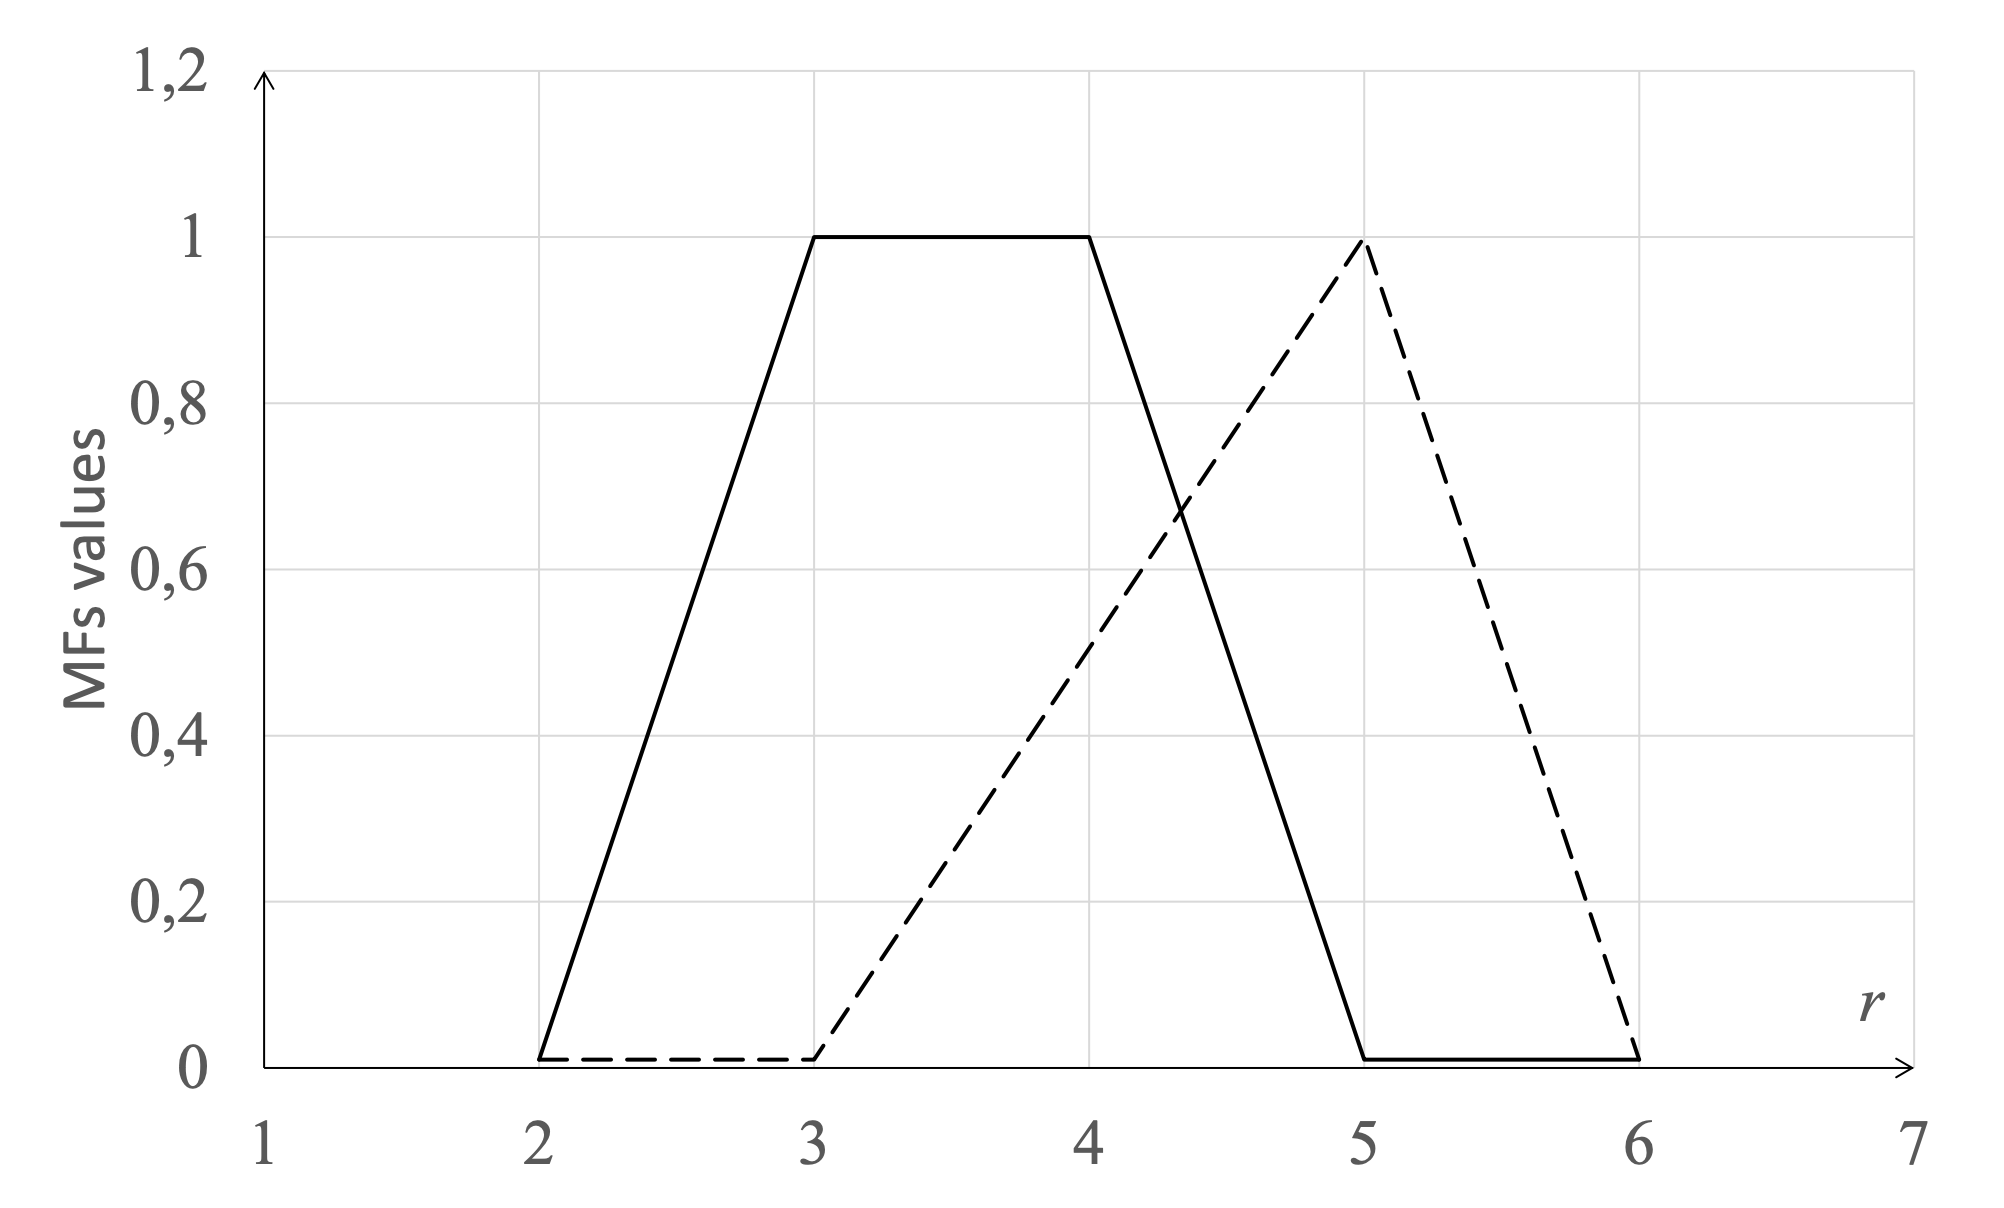
\includegraphics[width=1\textwidth]{image_2024-04-14_21-37-58.png}
    \caption{Нечіткі числа}
    \label{fig:my_label}
\end{figure}
\vspace{1ex}

Тоді сукупність
\begin{align*}
    &\tilde{F} = \left\{\left(\left(r, \mu_{F_{1}}(r)\right), \alpha_{1}\right), \left(\left(r, \mu_{F_{2}}(r)\right), \alpha_{2}\right): r \in \Re\right\} \\
    &= \left\{\left(F_{1}, \alpha_{1}\right), \left(F_{2}, \alpha_{2}\right)\right\} = \left\{\tilde{F}_{1}, \tilde{F}_{2}\right\}
\end{align*}
є НМТ-2, що розкладається за вторинними оцінками $\alpha_{1}$ та $\alpha_{2}$ на сукупність вкладених НМТ-2 $\tilde{F}_{1}$ та $\tilde{F}_{2}$ із сталими вторинними оцінками $\alpha_{1}$ та $\alpha_{2}$ відповідно. ФНТ-2 НМТ-2 $\tilde{F}$ задається як
\begin{equation*}
\eta_{\tilde{F}}(r, u)= \begin{cases}\alpha_{1}, & u=\mu_{F_{1}}(r), \\ \alpha_{2}, & u=\mu_{F_{2}}(r) ,\end{cases}
\end{equation*}

\subsection{Антагоністичні ігри з нечіткими виплатами}
Антагоністичні ігри з нечіткими виплатами мають наступний вигляд:
\begin{equation*}
G=\left(X_{i}, \tilde{f}_{i} \right)_{i \in I},
\end{equation*}
де $\tilde{f}_{i}, i \in I$ -- нечіткі числа. Розглянемо основні результати щодо нечітких матричних ігор.\cite{Larbani}

\subsubsection{Матричні ігри}
Матрична гра є скінченною грою двох осіб з нульовою сумою. У такій грі є два гравці: Гравець~I та Гравець~II. Гравець~I максимізує виграш, а Гравець~II мінімізує його. Оскільки це гра з нульовою сумою, її можна формально представити наступним чином:
\begin{equation*}
G=\left(X_{1}, X_{2}, A\right),
\end{equation*}
де $X_{1}=\{1,2, \ldots, m\}$ та $X_{2}=\{1,2, \ldots, n\}$ -- це множини чистих стратегій Гравців I та II відповідно; $A$ -- це матриця $m \times n$, яка представляє виграші Гравця I, які є програшами Гравця II.
\begin{equation*}
A=\left(\begin{array}{lll}
a_{11} & \ldots & a_{1 n} \\
\vdots & \ddots & \vdots \\
a_{m 1} & \ldots & a_{m n}
\end{array}\right),
\end{equation*}
Гравець І вибирає рядки, а Гравець~II вибирає стовпці матриці. Якщо гравці обирають пару чистих стратегій $(i, j)$, то Гравець І отримує винагороду $a_{i j}$, а Гравець~II отримує $-a_{i j}$.

\subsubsection{Нечіткі матричні ігри}
У цьому підрозділі представляється основна ідея найважливіших підходів для розв'язку матричних ігор з нечіткими виграшами. Матрична гра з нечіткими виграшами -- це скінчена гра з нульовою сумою для двох осіб із нечіткими виграшами. Її можна представити грою, подібною до звичайної матричної гри, з тією лише різницею, що матриця виграшів нечітка
\begin{equation*}
\begin{aligned}
& G=\left(S^{n}, S^{m}, \tilde{A}\right), \\
& \tilde{A}=\left(\tilde{a}_{i j}\right)_{\substack{1 \leqslant i \leqslant m \\
1 \leqslant j \leqslant n}}=\left(\begin{array}{llll}
\tilde{a}_{11} & \ldots & \tilde{a}_{1 n} \\
\vdots & \ddots & \vdots \\
\tilde{a}_{m 1} & \ldots & \tilde{a}_{m n}
\end{array}\right).
\end{aligned}
\end{equation*}

\subsubsection{Модель Кампоса}
Першу модель, що використовує ранжування нечітких чисел, представив Кампос. Кампос трансформує задачу пошуку розв'язку нечіткої матричної гри у наступну пару задач нечіткого лінійного програмування:
\begin{equation*}
\begin{aligned}
& \operatorname{Max} v, \qquad \qquad \quad \text { Min } w , \\
& \begin{array}{ll}p^{T} \tilde{A} \, \tilde{\geqslant} \, e w , & \tilde{A} q \,\tilde{\leqslant}\, e w \\e^{T} p=1, \quad  q \geqslant 0 , & e^{T} q=1, \quad q \geqslant 0 .\end{array}
\end{aligned}
\end{equation*}
Тут і далі $e$ представляє вектор відповідної розмірності, компоненти якого є одиницями. Використовуючи метод Ягера для вираження подвійних нечітких обмежень у термінах адекватності $\tilde{t}$ та $\tilde{k}$, пара задач оптимізації нечіткості перетворюється на наступну пару задач лінійного програмування:
\begin{equation*}
\begin{aligned}
\operatorname{Min} & \sum_{i=1}^{m} u_{i} , \\
& \sum_{i=1}^{m}\left(a_{i j}^{L}+a_{i j}+a_{i j}^{U}\right) u_{i} \geqslant 3-\left(t_{j}^{L}+t_{j}+t_{j}^{U}\right)(1-\alpha), \quad j=1, \ldots, n, \\
& \alpha \in[0,1], \quad u_{i} \geqslant 0, \quad i=1, \ldots, m
\end{aligned}
\end{equation*}
та
\begin{equation*}
\begin{aligned}
\operatorname{Max} & \sum_{j=1}^{n} s_{j} , \\
& \sum_{j=1}^{n}\left(a_{i j}^{L}+a_{i j}+a_{i j}^{U}\right) s_{j} \geqslant 3-\left(k_{i}^{L}+k_{i}+k_{i}^{U}\right)(1-\beta), \quad i=1, \ldots, m \\
& \beta \in[0,1], \quad s_{j} \geqslant 0, \quad j=1, \ldots, n
\end{aligned}
\end{equation*}
де $\tilde{a}_{i j}=\left(a_{i j}^{L}, a_{i j}, a_{i j}^{U}\right), \tilde{t}=\left(t_{j}^{L}, t_{j}, t_{j}^{U}\right)$ і $\tilde{k}=\left(k_{i}^{L}, k_{i}, k_{i}^{U}\right)$ є трикутними нечіткими числами (ТНЧ).
\subsubsection{Багатоцільовий підхід: модель Лі}
Лі використовував наступний порядок ранжування ТНЧ. 
Нехай $\tilde{a}=\left(a^{L}, a, a^{U}\right)$ та $\tilde{b}=\left(b^{L}, a, b^{U}\right)$ -- два ТНЧ.
$
\text{Тоді } \tilde{a} \,\tilde{\leqslant}\, \tilde{b} \text { якщо } a^{L} \leqslant b^{L}, a \leqslant b \text { та } a^{U}\leqslant b^{U}.
$

Нехай $\tilde{v}=\left(v^{L}, v, v^{U}\right)$ та $\tilde{w}=\left(w^{L}, w, w^{U}\right)$ -- два ТНЧ. Тоді $(\tilde{v}, \tilde{w})$ називається раціональним розв'язком гри, якщо існує $(\bar{p}, \bar{q}) \in S^{m} \times S^{n}$ такі, що

(i) $\bar{p}^{T} \tilde{A} q \geqslant \tilde{v}, \quad \forall q \in S^{n}$

(ii) $p^{T} \tilde{A} \bar{q} \leqslant \tilde{w}, \quad \forall p \in S^{m}$.\\
Позначимо $V=\{\tilde{v} / \tilde{v}$ виконує (i) $\}$ та $W=\{\tilde{w} / \tilde{w}$ виконує (ii) $\}$.\\
Елемент $\left(\tilde{v}^{}, \tilde{w}^{}\right) \in V \times W$ називається розв'язком гри, якщо

(1) $\tilde{v}^{*} \tilde{\geqslant} \tilde{v}, \quad \forall \tilde{v} \in V$,

(2) $\tilde{w}^{*} \tilde{\leqslant} \tilde{w}, \quad \forall \tilde{w} \in W$.

Задачу пошуку розв'язку гри можна тоді звести до наступної пари задач багатокритеріального програмування:
\begin{equation*}
\begin{aligned}
\operatorname{Max}, & \left(v^{L}, v, v^{U}\right) \\
& \sum_{i=1}^{m} a_{i j}^{L} p_{i} \geqslant v^{L}, \quad j=1, \ldots, n, \\
& \sum_{i=1}^{m} a_{i j} p_{i} \geqslant v, \quad j=1, \ldots, n, \\
& \sum_{i=1}^{m} a_{i j}^{U} p_{i} \geqslant v^{U}, \quad j=1, \ldots, n, \\
& e^{T} p=1, \quad p \geqslant 0
\end{aligned}
\end{equation*}
та
\begin{equation*}
\begin{aligned}
\operatorname{Min} , & \left(w^{L}, w, w^{U}\right) \\
& \sum_{j=1}^{n} a_{i j}^{L} q_{j} \leqslant w^{L}, \quad i=1, \ldots, m, \\
& \sum_{j=1}^{n} a_{i j} q_{j} \leqslant w, \quad i=1, \ldots, m, \\
& \sum_{j=1}^{n} a_{i j}^{U} q_{j} \leqslant w^{U}, \quad i=1, \ldots, m, \\
& e^{T} q=1, \quad q \geqslant 0 .
\end{aligned}
\end{equation*}

\subsubsection*{Модель Бектора}
Бектор використовує двоїстість у нечіткому лінійному програмуванні та перший індекс Ягера, щоб представити розв'язок матричної гри з нечіткими виграшами.

Нехай $\tilde{v}, \tilde{w}$ -- два нечітких числа. Тоді $(\tilde{v}, \tilde{w})$ називається {раціональним розв'язком гри}, якщо існує пара $x^{*} \in S^{m}, y^{*} \in S^{n}$ що задовольняє

(i) $x^{* T} \tilde{A} y \succcurlyeq \tilde{v}, \quad \forall y \in S^{n}$,

(ii) $x^{T} \tilde{A} y^{*} \preccurlyeq \tilde{w}, \quad \forall x \in S^{m}$.

Якщо $(\tilde{v}, \tilde{w})$ є раціональним розв'язком, то $\tilde{v}$ (відповідно, $\tilde{w}$ ) називається {прийнятним значенням} для Гравця I (відповідно, Гравця~II).

Нехай $T_{1}$ і $T_{2}$ -- набори всіх раціональних значень $\tilde{v}$ і $\tilde{w}$ для Гравців I та II відповідно, де $\tilde{v}, \tilde{w}$ є нечіткими числами. Нехай існують $\tilde{v}^{*} \in T_{1}$ та $\tilde{w}^{*} \in T_{2}$ такі, що

(i) $F\left(\tilde{v}^{*}\right) \geqslant F(\tilde{v}), \quad \forall \tilde{v} \in T_{1}$

(ii) $F\left(\tilde{w}^{*}\right) \leqslant F(\tilde{w}), \quad \forall \tilde{w} \in T_{2}$.

$F: N(R) \rightarrow R$ -- {функція дефазифікації}, де $N(R)$ -- множина дійсних нечітких чисел. Далі вводиться наступна пара задач нечіткого лінійного програмування для гравців I та II:
\begin{equation*}
\begin{cases}
\operatorname{Max} F(\tilde{v})\\
x^{T} \tilde{A} y \succcurlyeq \tilde{p} \tilde{v},\\ \forall y \in S^{n}, x \in S^{m}
\end{cases}
\end{equation*}
та
\begin{equation*}
\begin{cases}
\operatorname{Min} F(\tilde{w})\\
x^{T} \tilde{A} y \preccurlyeq \tilde{q} \tilde{w},\\ x \in S^{m}, y \in S^{n}
\end{cases}
\end{equation*}
де $x^{T} \tilde{A} y \succcurlyeq \tilde{p} \tilde{v}$ і $x^{T} \tilde{A} y \preccurlyeq \tilde{q} \tilde{w }$
-- двоїсті нечіткі нерівності з адекватністю $\tilde{p}$ та $\tilde{q}$ відповідно. 

Звідси задачі перетворюється на наступну чітку пару задач:
\begin{equation*}
\begin{aligned}
&\text{Max } V, \\
&\text{} \begin{cases}
\sum_{i=1}^{m} F\left(\tilde{a}_{i j}\right) x_{i} \geqslant V+(1-\gamma) F(\tilde{p}), & j=1,\dots,n, \\
\sum_{i=1}^{m} x_{i}=1, x \geqslant 0, 0 \leqslant \gamma \leqslant 1
\end{cases}
\end{aligned}
\end{equation*}
та
\begin{equation*}
\begin{aligned}
&\text{Min } W , \\
&\text{} \begin{cases}
\sum_{j=1}^{n} F\left(\tilde{a}_{i j}\right) y_{j} \leqslant W+(1-\rho) F(\tilde{q}), & i=1,\dots,m, \\
\sum_{j=1}^{n} y_{j}=1,
y \geqslant 0,
0 \leqslant \rho \leqslant 1
\end{cases}
\end{aligned}
\end{equation*}

\subsubsection{Модель Лю та Као}

Лю та Као розробили метод розв'язання матричних ігор з нечіткими виграшами на основі принципу узагальнення. Розглянемо нечітку матричну гру. Тоді задача для Гравця I (Гравець~II) полягає знаходженні оптимального розв'язоку задачі. Використовуючи принцип узагальнення, Лю та Као визначають цінність гри як нечітке число $\tilde{Z}$ з такою функцією належності:
\begin{equation*}
\mu_{\tilde{Z}}(z)=\operatorname{Sup}_{a_{i j}} \operatorname{Min}\left\{\mu_{\tilde{a}_{i j}}\left(a_{i j}\right), \quad \forall i, j / z=Z(a)\right\} .
\end{equation*}
Для фіксованого значення рівня перерізу $\alpha$ верхня межа $\tilde{Z}_{\alpha}^{U}$ і нижня межа $\tilde{Z}_{\alpha}^{L} $ з $\tilde{Z}$ обчислюються шляхом розв'язання наступної пари дворівневих задач, відповідно,
\begin{equation*}
\begin{aligned}
\tilde{Z}_\alpha^U= & \operatorname{Max}_{\left(a_{i j}\right)_\alpha^L \leqslant a_{i j} \leqslant\left(a_{i j}\right)_\alpha^U, \quad \forall i, j} \operatorname{Max}_p v \\
& \left\{\begin{aligned}
&\sum_{i=1}^m a_{i j} p_i \geqslant v, \quad j=1, \ldots, n, \\
&\sum_{i=1}^m p_i=1, \\
&p_i \geqslant 0, \quad i=1, \ldots, m
\end{aligned}\right.
\end{aligned}
\end{equation*}
та
\begin{equation*}
\begin{aligned}
\tilde{Z}_\alpha^L= & \operatorname{Min}_{\left(a_{i j}\right)_\alpha^L \leqslant a_{i j} \leqslant\left(a_{i j}\right)_\alpha^U, \forall i, j} \operatorname{Max}_p v \\
& \left\{\begin{aligned}
&\sum_{i=1}^m a_{i j} p_i \geqslant v, \quad j=1, \ldots, n, \\
&\sum_{i=1}^m p_i=1, \\
&p_i \geqslant 0, \quad i=1, \ldots, m 
\end{aligned}\right.
\end{aligned}
\end{equation*}
Аналогічну пару дворівневих задач можна сформулювати для Гравця II. Тоді використовуючи заміну змінної $t_{i j}=a_{i j} p_{i}$ та $l_{i j}=a_{i j} q_{j}$ отримуємо таку пару задач лінійного програмування:
\begin{equation*}
\begin{aligned}
& \tilde{Z}_{\alpha}^{U}= \operatorname{Max} v, \\
& \qquad\left\{\begin{aligned}
& \sum_{i=1}^{m} t_{i j} \geqslant v, \quad j=1, \ldots, n, \\
& \sum_{i=1}^{m} p_{i}=1, \\
& \left(a_{i j}\right)_{\alpha}^{L} p_{i} \leqslant t_{i j} \leqslant\left(a_{i j}\right)_{\alpha}^{U} p_{i}, \quad i=1, \ldots, m,\quad j=1, \ldots, n, \\
& p_{i} \geqslant 0, t_{i j}, v \quad i=1, \ldots, m, \quad j=1, \ldots, n .
\end{aligned}\right.
\end{aligned}
\end{equation*}
та
\begin{equation*}
\begin{aligned}
& \tilde{Z}_{\alpha}^{L}= \operatorname{Min} u, \\
& \qquad\left\{\begin{aligned}
& \sum_{j=1}^{n} l_{i j} \leqslant u, \quad i=1, \ldots, m, \\
& \sum_{j=1}^{n} q_{j}=1, \\
& \left(a_{i j}\right)_{\alpha}^{L} q_{j} \leqslant l_{i j} \leqslant\left(a_{i j}\right)_{\alpha}^{U} q_{j}, \quad i=1, \ldots, m,\quad j=1, \ldots, n, \\
& q_{j} \geqslant 0, l_{i j}, u \quad i=1, \ldots, m,\quad j=1, \ldots, n .
\end{aligned}\right.
\end{aligned}
\end{equation*}
Цільове значення $\tilde{Z}_{\alpha}^{L}$ разом із $\tilde{Z}_{\alpha}^{U}$, становить $\alpha$-переріз $\left[\tilde{Z}_{\alpha}^{L}, \tilde{Z}_{\alpha}^{U}\right]$, де значення $\tilde {Z}$ нечіткої гри лежить на зазначеному $\alpha$-рівні. Подібне перетворення можна застосувати до пари задач, пов'язаних з Гравцем II. Це показує, що нечітке значення, розраховане для двох гравців, однакове. Зверніть увагу, що більшість підходів до розв'язання гри не забезпечують однакові нечіткі або чіткі значення для обох гравців. Нехай $R(z)=\left(Z_{\alpha}^{U}\right)^{-1}$ та $L(z)=\left(Z_{\alpha}^{L}\right) ^{-1}$ -- права та ліва функції форми нечіткого значення $\tilde{Z}$, тоді $\tilde{Z}$ можна отримати як
\begin{equation*}
\mu_{\tilde{z}}(z)=\left\{\begin{array}{ll}
L(z), & z_{\alpha=0}^{L} \leqslant z \leqslant z_{\alpha=1}^{L}, \\
1, & z_{\alpha=1}^{L} \leqslant z \leqslant z_{\alpha=1}^{U}, \\
R(z), & z_{\alpha=1}^{U} \leqslant z \leqslant z_{\alpha=0}^{L} .
\end{array} .\right.
\end{equation*}
У більшості випадків рівняння $R(z)=\left(Z_{\alpha}^{U}\right)^{-1}$ і $L(z)=\left(Z_{\alpha}^{L}\right)^{-1}$ неможливо знайти аналітично. Однак для різних рівнів можливостей $\alpha, \tilde{Z}_{\alpha}^{L}$ і $\tilde{Z}_{\alpha}^{U}$ можна обчислити для наближено для форм $R(z)$ і $L(z)$ відповідно.

\section{МАТРИЧНА ГРА З НЕЧІТКИМИ МНОЖИНАМИ СТРАТЕГІЙ ГРАВЦІВ}

\subsection{Класична матрична гра}Матрична гра -- це двоосібна гра з скінченною кількістю стратегій та нульовою сумою виграшів. Вона може бути формально представлена у нормальній формі $\langle I, J, A(I, J)\rangle$, де $I=\{1, \ldots, |I|\}$ та $J=\{1, \ldots, |J|\}$ -- скінчені множини чистих стратегій гравців 1 та 2 відповідно; $A(I, J)=\left(a_{ij}\right)_{i \in I, j \in J}$ -- матриця виграшів, яка представляє виграші $a_{ij}$ гравця 1 в ситуації $(i, j)$, коли гравці 1 та 2 обирають стратегії $i \in I$ та $j \in J$ відповідно; |.| -- це потужність множини. Для зручності подальшого викладу множини $I$ та $J$ чистих стратегій зазначаються далі як параметри у матриці виграшів. Оскільки гра має нульову суму виграшів, гравець 2 в ситуації $(i, j)$ отримує виграш $-a_{ij}$. Значення $a_{ij}$ також зручно називати програшом гравця 2. В цьому випадку ми припускаємо, що гравець 1 максимізує свій виграш, тоді як гравець 2 мінімізує свій програш.

Сідлова точка гри $\langle I, J, A(I, J)\rangle$ -- це ситуація $\left(i^*, j^*\right)$, $i^* \in I$ та $j^* \in J$, для якої виконуються нерівності $a_{ij^*} \leq a_{i^*j^*} \leq a_{i^*j}$ для всіх $i \in I$ та $j \in J$. Вибір стратегій $i^*$ та $j^*$ обома гравцями 1 та 2 відповідно, здається раціональним. Справді, відхилення від цих стратегій не вигідне для кожного з них окремо, а також для обох разом. Гра $\langle I, J, A(I, J)\rangle$ не завжди має сідлову точку в чистих стратегіях. Якщо її немає, гравці можуть використовувати змішані стратегії, які є розподілами ймовірностей на множинах чистих стратегій. Тоді ми отримуємо матричну гру $G(I, J)=\langle X(I), Y(J), A(I, J)\rangle$ у змішаних стратегіях, де $X(I)=\{x=\left(x_i\right)_{i \in I}: x_i \geq 0$,
$i \in I; \sum_{i \in I} x_i=1\}, Y(J)=\left\{y=\left(y_j\right)_{j \in J}:\right.$ $\left.y_j \geq 0, j \in J ; \sum_{j \in J} y_j=1\right\}$ -- множини змішаних стратегій $x$ та $y$ гравців 1 та 2 відповідно. У змішаній стратегії $x=\left(x_i\right)_{i \in I}$, гравець 1 обирає чисту стратегію $i \in I$ з ймовірністю $x_i \in[0,1]$. Аналогічно, у змішаній стратегії $y=\left(y_j\right)_{j \in J}$, гравець 2 обирає чисту стратегію $j \in J$ з ймовірністю $y_j \in[0,1]$. У матричній грі $G(I, J)$ у змішаних стратегіях, очікуваний виграш гравця 1, який дорівнює очікуваному програшу гравця 2, дорівнює $x A(I, J) y^T$. Сідлова точка $(\hat{x}, \hat{y}), \hat{x} \in X, \hat{y} \in Y$ матричної гри $G(I, J)$ у змішаних стратегіях характеризується наступними нерівностями:
\begin{equation*}
x A(I, J) \hat{y}^T \leq \hat{x} A(I, J) \hat{y}^T \leq \hat{x} A(I, J) y^T, x \in X(I), y \in Y(J)
\end{equation*}
і може бути знайдена як розв'язок пари двоїстих задач:
\begin{align}\label{zadah}
& Z(G(I, J))=\max v \\
& \sum_{i \in I} a_{ij} x_i \geq v, j \in J ; \sum_{i \in I} x_i=1 \\
& x_i \geq 0, i \in I, v \in \Re
\end{align}
та
\begin{align}
& Z(G(I, J))=\min w \\
& \sum_{j \in J} a_{ij} y_j \leq w, i \in I ; \sum_{j in J} y_j=1 ;\\
& y_j \geq 0, j \in J, u \in \Re .
\end{align}
У цих задачах змінні $u$ та $v$ приймають значення обох знаків. Множина сідлових точок $(\hat{x}, \hat{y})$ не є порожньою. Значення матричної гри $G(I, J)$ у змішаних стратегіях має форму $Z(G(I, J))=\hat{x} A(I, J) \hat{y}^T$.

\subsection{Постановка задачі}
Розглянемо матричну гру у нормальній формі $\langle M, N, A(M, N)\rangle$ з матрицею виграшу $A(M, N)=\left(A_{i j}\right)_{i \in M, j \in N}$, де $M=\{1, \ldots, m\}$ і $N= \{1, \ldots, n\}$ -- скінченні набори чистих стратегій гравців 1 і 2 відповідно. Нехай $\tilde{M}=\left\{\left(i, \mu_{\tilde{M}}(i)\right): i \in M\right\}$ та $\tilde{N}=\left\{\left(j, \mu_{\tilde{N}}(j)\right): j \in N\right\}$ є деякими нечіткими множинами (НМ), з ФН $\mu_{\tilde{M}}(i), i \in M$ та $\mu_{\tilde{N}}(j), j \in N$ на множинах $M$ та $N$ чистих стратегій гравців 1 і 2 відповідно. Назвемо $\tilde{M}$ та $\tilde{N}$ НМ стратегій. Припустимо, що НМ $\tilde{M}$ та $\tilde{N}$ є нормальними, тобто
\begin{equation*}
\max _{i \in M} \mu_{\tilde{M}}(i)=1, \max _{j \in N} \mu_{\tilde{N}}(j)=1.
\end{equation*}
Виникає наступне питання: <<Яке значення матричної гри у випадку, коли множини стратегій гравців є нечіткими?>> Представляємо таку гру у нормальній формі $\langle\tilde{M}, \tilde{N}, A(M, N)\rangle$. Інше природне питання: <<Коли є потреба в таких операціях?>> Для відповіді на це питання розглянемо наступні приклади. Припустимо, що особа приймаюча рішення (ОПР) намагається передбачити результат конфлікту між двома гравцями, який може бути сформульований як деяка класична матрична гра з чіткими наборами стратегій гравців та чіткою матрицею виграшів. Проблема полягає в тому, що ОПР знає лише ступені належності стратегій гравців до деяких НМ їхніх стратегій. Також ОПР знає лише числа, які є елементами матриці виграшів. Наступний приклад -- це випадок матричної гри, за умови, що кожен гравець знає лише ступені належності стратегій партнерів до деякої НМ. У цьому випадку прогнозування значення гри може бути проблемою для обох гравців.


\subsection{Основна ідея}
Спочатку узагальнимо задачу для випадку довільних підмножин $I \subseteq M, I \neq \emptyset$ та $J \subseteq N, J \neq \emptyset$ стратегій. У цьому випадку матриця виграшу $A(I, J)=\left(A_{i j}\right)_{i \in I, j \in J}$ є відповідною підматрицею матриці $A(M, N)=\left(A_{i j}\right)_{i \in M, j \in N}$.

Для кожного фіксованого $z \in \Re$, розглянемо відображення $V^{z}: 2^{M \times N} \rightarrow\{0,1\}$, задане як
\begin{equation}\label{formul}
V^{z}(I, J) = 
\begin{cases} 
1, & z = Z(F(I, J)), \\
0, & z \neq Z(F(I, J)),
\end{cases}
\end{equation}

де $I \subseteq M, J \subseteq N$.
Числа $Z(F(I, J))$, є значенням гри $F(I, J)=\langle I, J, A(I, J)\rangle$ у змішаних стратегіях, обчислюються шляхом розв'язання пари задач (\ref{zadah}). Відображення $V^{z}$ співставляє кожній парі підмножин $I \subseteq M$ і $J \subseteq N$ стратегій зі значенням ФН
\begin{equation*}
\mu_{Z(F(I, J))}(z)=V^{z}(I, J), z \in \operatorname{supp}\left(Z(F(I, J))=\left\{z \in \Re: V^{z}(I, J) \neq 0\right\}\right),
\end{equation*}
числа чіткої множини
\begin{equation*}
Z(F(I, J))=\left\{\left(z, \mu_{Z(F(I, J))}(z)\right): z \in \Re\right\},
\end{equation*}
яке представляє значення гри $F(I, J)=\langle I, J, A(I, J)\rangle$ у змішаних стратегіях.

Позначемо $\operatorname{supp}(Z(F(I, J))$ носій чіткої множини $Z(F(I, J))$. Підмножини $I \subseteq M$ та $J \subseteq N$ стратегій є параметрами задач, від яких залежать як набори змінних, так і набори обмежень. Тому, для зручності подальшого викладу, представляємо у наступній формі:

\begin{equation*}
\begin{array}{r}
Z(F(I, J))=\max v \\
\sum_{i \in M} p_{i j} \geq v, j \in J ; \sum_{i \in M} x_{i}=1 ; \\
p_{i j} = Ax_{i}, i \in M, j \in N ; \\
x_{i} \geq 0, i \in M ; v \in \Re ; p_{i j} \geq 0, i \in M, j \in N \\
x_{i}=0, i \notin I ;
\end{array}
\end{equation*}
та
\begin{equation*}
\begin{array}{r}
Z(F(I, J))=\min w \\
\sum_{j \in N} p_{i j} \leq w, i \in I ; \sum_{j \in N} y_{j}=1 ; \\
q_{i j} = Ay_{j}, i \in M, j \in N ;\\
y_{j} \geq 0, j \in N ; w \in \Re ; q_{i j} \geq 0, i \in M, j \in N \\
y_{j}=0, j \notin J,
\end{array}
\end{equation*}
відповідно. Кількість обмежень залежить від підмножин $I \subseteq M$ та $J \subseteq N$ і не залежить від кількості змінних.

Далі, ми узагальнюємо формули (\ref{formul}) до випадку НМ стратегій $\tilde{M}$ та $\tilde{N}$. Ми позначаємо через $W$ значення гри $\langle\tilde{M}, \tilde{N}, A(M, N)\rangle$ і через $M_{W}(z), z \in \Re$ відповідний ФН. У цьому випадку, для кожного фіксованого $z=z^{*}$, значення ФН $M_{W}\left(z^{*}\right)$ співпадає з образом $V^{z^{*}}(\tilde{M}, \tilde{N})$ пари НМ $\tilde{M}$ та $\tilde{N}$ при відображенні $V^{z^{*}}$, тобто,
\begin{equation*}
M_{W}\left(z^{*}\right)=V^{z^{*}}(\tilde{M}, \tilde{N}).
\end{equation*}
Образ пари НМ $\tilde{M}$ та $\tilde{N}$ при відображенні $V^{z^{*}}: 2^{M \times N} \rightarrow[0,1]$ є НМ
\begin{equation*}
V^{z^{*}}(\tilde{M}, \tilde{N})=\left\{\left(u, \mu_{V^{z^{*}}(\tilde{M}, \tilde{N})}\right): u \in[0,1]\right\}
\end{equation*}
з ФН
\begin{equation*}
    \mu_{V^{z^{*}}(\tilde{M}, \tilde{N})}(u)=\max \left\{\min \{\alpha, \beta\}: \alpha, \beta \in[0,1]; u=V^{z^{*}}\left(I_{\alpha}, J_{\beta}\right), u \in[0,1]\right\}.
\end{equation*}
У цій формулі, $I_{\alpha}=\left\{i \in M: \mu_{\tilde{M}}(i) \geq \alpha\right\}$ є $\alpha$-перерізом, $\alpha \in[0,1]$ НМ $\tilde{M}=\left\{\left(i, \mu_{\tilde{M}}(i)\right): i \in M\right\}$ стратегій, і $J_{\beta}=\left\{j \in N: \mu_{\tilde{N}}(j) \geq \beta\right\}$ є $\beta$-перерізом, $\beta \in[0,1]$ НМ $\tilde{N}=\left\{\left(j, \mu_{\tilde{N}}(j)\right): j \in N\right\}$ стратегій;
\begin{equation*}
V^{z^{*}}\left(I_{\alpha}, J_{\beta}\right)=\mu_{Z\left(I_{\alpha}, J_{\beta}\right)}\left(z^{*}\right)
\end{equation*}
є образом пари перерізів $I_{\alpha}$ та $J_{\beta}$ множин НМ стратегій при відображенні $V^{z^{*}}$. Значення $V^{z^{*}}\left(I_{\alpha}, J_{\beta}\right)$ дорівнює значенню ФН $\mu_{Z\left(I_{\alpha}, J_{\beta}\right)}\left(z^{*}\right)$
для НМ $Z\left(I_{\alpha}, J_{\beta}\right)$ при $I=I_{\alpha}$ та $J=J_{\beta}$, $\alpha, \beta \in[0,1]$.

\textbf{Зауваження 2.1.} Нехай $\Omega_{\tilde{M}}=\left\{\mu_{\tilde{M}}(i): i \in M\right\}$ та\\ $\Omega_{\tilde{N}}=\left\{\mu_{\tilde{N}}(j): j \in N\right\}$ є наборами значень ступенів належності НМ $\tilde{M}=\left\{\left(i, \mu_{\tilde{M}}(i)\right): i \in M\right\}$ та $\tilde{N}=\left\{\left(j, \mu_{\tilde{N}}(j)\right): j \in N\right\}$ стратегій, відповідно. Зауважимо, що потужності множин $\Omega_{\tilde{M}}$ та $\Omega_{\tilde{N}}$ є $\left|\Omega_{\tilde{M}}\right| \leq m$ та $\left|\Omega_{\tilde{N}}\right| \leq n$, відповідно. Ясно, що при отриманні $\alpha$-перерізів $I_{\alpha}, \alpha \in[0,1]$ НМ $\tilde{M}$ та $\beta$-перерізів $J_{\beta}, \beta \in[0,1]$ НМ $N$ ми можемо припустити, що $\alpha \in \Omega_{\tilde{M}}$ та $\beta \in \Omega_{\tilde{N}}$ замість $\alpha \in[0,1]$ та $\beta \in[0,1]$. Також зазначимо, що $1 \in \Omega_{\tilde{M}}$ та $1 \in \Omega_{\tilde{N}}$.

Таким чином, за фіксованим $z=z^{*}$, значення ФН $M_{W}\left(z^{*}\right)$ формують НМ $\operatorname{НМ}\left\{\left(u, \mu_{M_{W}\left(z^{*}\right)}(u)\right): u \in\{0,1\}\right\}$ на $\{0,1\}$ для ФН
\begin{equation*}
\begin{array}{r}
\mu_{M_{\tilde{W}}\left(z^{*}\right)}(u)=\max \left\{\min \{\alpha, \beta\}: \alpha \in \Omega_{\tilde{M}}, \beta \in \Omega_{\tilde{N}}, u=\mu_{Z\left(I_{\alpha}, J_{\beta}\right)}\left(z^{*}\right)\right\}, \\
u \in \operatorname{supp}\left(M_{\tilde{W}}\left(z^{*}\right)\right)=\left\{u \in[0,1]: u=\mu_{Z\left(I_{\alpha}, J_{\beta}\right)}\left(z^{*}\right), \alpha \in \Omega_{\tilde{M}}, \beta \in \Omega_{\tilde{N}}\right\}.
\end{array}
\end{equation*}
Тому ми робимо висновок, що $\tilde{W}$ є НМ на $\Re$ для ФН, значення якої формують НМ на $[0,1]$. Тоді, $\tilde{W}$ є НМТ-2 на $\Re$. У спосіб вертикальних зрізів НМТ-2 $\tilde{W}$ на $\Re$ має форму:
\begin{equation*}
\tilde{W}=\left\{\left(z, M_{\tilde{W}}(z)\right): z \in \Re\right\}=\left\{\left(z,\left\{\left(u, \mu_{M_{\tilde{W}}(z)}(u)\right): u \in U_{z}\right\}\right): z \in \Re\right\}.
\end{equation*}
У цій формулі, $\mu_{M_{\tilde{W}}(z)}(u), u \in U_{z} \subseteq\{0,1\}$ є ФН НМ\\ $M_{\tilde{W}}(z) = \left\{\left(u, \mu_{M_{\tilde{W}}(z)}(u)\right): u \in U_{z}\right\}$ значень нечіткого ступеня належності числа $z \in \Re$ до НМТ-2 $\tilde{W}$, і $U_{z}=\operatorname{supp}\left(M_{\tilde{W}}(z)\right)$ є набором первинних ступенів належності, де $\operatorname{supp}\left(M_{\tilde{W}}(z)\right)$ позначає носій НМ $M_{\tilde{W}}(z)$ для $z \in \Re$. Також можемо характеризувати НМТ-2 $\tilde{W}$ за допомогою ФНТ-2 $\eta_{\tilde{W}}(z, u)=\mu_{M_{\tilde{W}}(z)}(u), u \in U_{z}$ і $\eta_{\tilde{W}}(z, u)=0, u \notin U_{z}$. Це висновок дозволяє ввести наступне поняття.
\\
\\

\textbf{Визначення 2.1.} Під значенням гри $\langle\tilde{M}, \tilde{N}, A(M, N)\rangle$ для НМ стратегій $\tilde{M}$ і $\tilde{N}$ розуміється НМТ-2
\begin{equation*}
\tilde{W}=\left\{\left((z, u), \eta_{\tilde{W}}(z, u)\right): u \in\{0,1\}, z \in \Re\right\},
\end{equation*}
на $\Re$ для ФНТ-2

\begin{equation*}
\eta_{\tilde{W}}(z, u)=\left\{\begin{array}{cc}
\max _{\alpha \in \Omega_{\tilde{M}}, \beta \in \Omega_{\tilde{N}}}\left\{\min \{\alpha, \beta\}: u=\mu_{Z\left(I_{\alpha}, J_{\beta}\right)}(z)\right\}, & u \in U_{z} ;\\
0, & u \notin U_{z} .
\end{array}\right.
\end{equation*}
У цьому визначенні,
\begin{equation*}
U_{z}=\left\{u \in\{0,1\}: u=\mu_{Z\left(I_{\alpha}, J_{\beta}\right)}(z), \alpha \in \Omega_{\tilde{M}}, \beta \in \Omega_{\tilde{N}}\right\}
\end{equation*}
є набором первинних ступенів належності $u$ зі строго додатними вторинними оцінками $\eta_{\tilde{W}}(z, u)$, який збігається з носієм $\operatorname{supp}\left(M_{\tilde{W}}(z)\right)$ НМ $M_{\tilde{W}}(z)$ нечітких ступенів належності елемента $z \in \Re$;
\begin{equation*}
\mu_{Z\left(F\left(I_{\alpha}, J_{\beta}\right)\right)}(z)=
\begin{cases} 
1, & z = Z\left(F\left(I_{\alpha}, J_{\beta}\right)\right), \\
0, & z \neq Z\left(F\left(I_{\alpha}, J_{\beta}\right)\right))
\end{cases}
\end{equation*}
є ФН чіткої множини
\begin{equation*}
Z\left(F\left(I_{\alpha}, J_{\beta}\right)\right)=\left\{\left(z, \mu_{Z\left(F\left(I_{\alpha}, J_{\beta}\right)\right)}(z)\right): z \in \Re\right\},
\end{equation*}
яке визначає значенням матричної гри $F\left(I_{\alpha}, J_{\beta}\right)$ для наборів стратегій $I_{\alpha}$ і $J_{\beta}$ для $I=I_{\alpha}$ і $J=J_{\beta}$).
\begin{equation*}
I_{\alpha}=\left\{i \in M: \mu_{\tilde{M}}(i) \geq \alpha\right\} \text { та } J_{\beta}=\left\{j \in N: \mu_{\tilde{N}}(j) \geq \beta\right\}
\end{equation*}
є перерізами НМ $\tilde{M}=\left\{\left(i, \mu_{\tilde{M}}(i)\right): i \in M\right\}$ та $\tilde{N}=\left\{\left(j, \mu_{\tilde{N}}(j)\right): j \in N\right\}$ стратегій відповідно;

$\Omega_{\tilde{M}}=\left\{\mu_{\tilde{M}}(i): i \in M\right\}$ та $\Omega_{\tilde{N}}=\left\{\mu_{\tilde{N}}(j): j \in N\right\}$ є наборами значень ступенів належності $\mu_{\tilde{M}}(i), i \in M$ і $\mu_{\tilde{N}}(j), j \in N$ НМ $\tilde{M}$ та $\tilde{N}$ стратегій відповідно.

\subsection{Ціна гри з нечіткими множинами стратегій гравців}
\subsubsection{Декомпозиція нечіткої множини типу-2 значення гри}
Теорема 2.1 обґрунтовує можливісь розбиття НМТ-2 значення гри з нечіткими множинами стратегій на сукупність вкладених НМТ-2 зі сталими вторинними оцінками (Визначення 2.1).

\textbf{Теорема 2.1.} НМТ-2 значення $\tilde{W}$ матричної гри $\langle\tilde{M}, \tilde{N}, A(M, N)\rangle$ для НМ стратегій розкладається за вторинними оцінками $\min \{\alpha, \beta\}$ на сукупність
\begin{equation*}
\tilde{W}=\left\{\tilde{W}^{e 2}\left(I_{\alpha}, J_{\beta}\right): \alpha \in \Omega_{\tilde{M}}, \beta \in \Omega_{\tilde{N}}\right\}
\end{equation*}

вкладених НМТ-2
\begin{equation*}
\tilde{W}^{e 2}\left(I_{\alpha}, J_{\beta}\right)=\left\{\left(Z\left(F\left(I_{\alpha}, J_{\beta}\right)\right), \min \{\alpha, \beta\}\right)\right\},
\end{equation*}
де $Z\left(F\left(I_{\alpha}, J_{\beta}\right)\right)=\left\{\left(z, \mu_{Z\left(F\left(I_{\alpha}, J_{\beta}\right)\right)}(z)\right): z \in \Re\right\}$ є вкладеним НМТ-1. Це число, яке є значенням матричної гри $F\left(I_{\alpha}, J_{\beta}\right)=\left\langle I_{\alpha}, J_{\beta}, A\left(I_{\alpha}, J_{\beta}\right)\right\rangle$ для чітких множин $I_{\alpha}, \alpha \in \Omega_{\tilde{M}}$ та $J_{\beta}, \beta \in \Omega_{\tilde{N}}$ стратегій.

Доведення. НМТ-2 значення задається як $\tilde{W}=\left\{\left((z, u), \eta_{\tilde{W}}(z, u)\right):\\ u \in\right.$ $\{0,1\}, z \in \Re\}$. Звідси, отримуємо
\begin{equation*}
\begin{array}{l}
\tilde{W}=\left\{\left\{\left((z, u), \max \left\{\min \{\alpha, \beta\}: \alpha \in \Omega_{\tilde{M}}, \beta \in \Omega_{\tilde{N}},\right.\right.\right.\right. \\
\left.\left.\left.\left.u=\mu_{Z\left(I_{\alpha}, J_{\beta}\right)}(z)\right\}\right): u \in U_{z}\right\} \bigcup\left\{((z, u), 0): u \in\{0,1\} \backslash U_{z}\right\}: z \in \Re\right\} ,
\end{array}
\end{equation*}
Оскільки Зауваження 1.2 дозволяє ігнорувати пари $(z, u)$, що мають вторинні оцінки, що дорівнюють нулю, робимо висновок, що 
\begin{equation*}
\begin{array}{l}
    \tilde{W}=\{\left((z, u), \max \left\{\min \{\alpha, \beta\}: \alpha \in \Omega_{\tilde{M}}, \beta \in \Omega_{\tilde{N}}, u=\mu_{Z\left(I_{\alpha}, J_{\beta}\right)}(z)\right\}\right):\\
    u \in U_{z}, z \in \Re\},
\end{array}
\end{equation*}
та,
\begin{equation*}
\tilde{W}=\left\{\left(z,\left\{\left(\mu_{Z\left(I_{\alpha}, J_{\beta)}\right)}(z), \min \{\alpha, \beta\}\right): \alpha \in \Omega_{\tilde{M}}, \beta \in \Omega_{\tilde{N}}\right\}\right): z \in \Re\right\},
\end{equation*}
Далі, групуючи елементи, отримуємо
\begin{equation*}
\begin{aligned}
\tilde{W}= & \left\{\left(z,\left(\mu_{Z\left(F\left(I_{\alpha}, J_{\beta}\right)\right)}(z), \min \{\alpha, \beta\}\right)\right): \alpha \in \Omega_{\tilde{M}}, \beta \in \Omega_{\tilde{N}}, z \in \Re\right\}= \\
& \left\{\left\{\left(\left(z, \mu_{Z\left(F\left(I_{\alpha}, J_{\beta}\right)\right)}(z)\right), \min \{\alpha, \beta\}\right): z \in \Re\right\}: \alpha \in \Omega_{\tilde{M}}, \beta \in \Omega_{\tilde{N}}\right\} ,
\end{aligned}
\end{equation*}
Звідси
\begin{equation*}
\tilde{W}=\left\{\left(Z\left(F\left(I_{\alpha}, J_{\beta}\right)\right), \min \{\alpha, \beta\}\right): \alpha \in \Omega_{\tilde{M}}, \beta \in \Omega_{\tilde{N}}\right\},
\end{equation*}
Доведення Теореми 2.1 завершено.

Теорема 2.1 дозволяє представити НМТ-2 $\tilde{W}$ у більш зручній формі для обчислення та інтерпретації. Згідно з Зауваженням 2.1, НМТ-2 $\tilde{W}$ можна інтерпретувати як сукупність значень $Z\left(F\left(I_{\alpha}, J_{\beta}\right)\right.$ чітких ігор $F\left(I_{\alpha}, J_{\beta}\right)$ для відповідних чітких множин $I_{\alpha}, \alpha \in \Omega_{\tilde{M}}$ і $J_{\beta}, \beta \in \Omega_{\tilde{N}}$ стратегій зі ступенем істинності $Z\left(F\left(I_{\alpha}, J_{\beta}\right)\right)$, який дорівнює $\min \{\alpha, \beta\}$.

Позначимо
\begin{equation*}
\Omega=\left\{\min \{\alpha, \beta\}: \alpha \in \Omega_{\tilde{M}}, \beta \in \Omega_{\tilde{N}}\right\}
\end{equation*}
\noindent множину вторинних оцінок НМТ-2 значення $\tilde{W}$ гри $\langle\tilde{M}, \tilde{N}, A(M, N)\rangle$. Наслідок 2.1 стверджує, що НМТ-2 $\tilde{W}$ може бути безпосередньо розкладено за набором $\Omega$ вторинних оцінок.

\noindent \textbf{Наслідок 2.1.} НМТ-2 значення $\tilde{W}$ матричної гри $\langle\tilde{M}, \tilde{N}, A(M, N)\rangle$ для НМ стратегій розкладається за вторинними оцінками $\gamma \in \Omega$ на сукупність

\begin{equation*}
\tilde{W}=\left\{\left(W_{\gamma}^{e 1}, \gamma\right): \gamma \in \Omega\right\}
\end{equation*}

\noindent вкладених НМТ-2

\begin{equation*}
\tilde{W}_{\gamma}^{e 2}=\left\{\left(W_{\gamma}^{e 1}, \gamma\right)\right\}.
\end{equation*}
Для кожного $\gamma \in \Omega$, чітка множина

\begin{equation*}
W_{\gamma}^{e 1}=\bigcup_{\alpha \in \Omega_{\tilde{M}}, \beta \in \Omega_{\tilde{N}}: \min \{\alpha, \beta\}=\gamma} Z\left(F\left(I_{\alpha}, J_{\beta}\right)\right)
\end{equation*}

\noindent є сукупністьм $Z\left(F\left(I_{\alpha}, J_{\beta}\right)\right)$, які є значеннями чітких матричних ігор $F\left(I_{\alpha}, J_{\beta}\right)$ для наборів стратегій $I_{\alpha}$ та $J_{\beta}$ $\alpha \in \Omega_{\tilde{M}}$ та $\beta \in \Omega_{\tilde{N}}$ з $\min \{\alpha, \beta\}=\gamma$.

\noindent Доведення. Передбачається, що
\begin{equation*}
\tilde{W}=\left\{\left(Z\left(F\left(I_{\alpha}, J_{\beta}\right)\right), \min \{\alpha, \beta\}\right): \alpha \in \Omega_{\tilde{M}}, \beta \in \Omega_{\tilde{N}}\right\}.
\end{equation*}

\noindent Згідно з Зауваженням 2.1, кожен елемент цієї сукупності може бути інтерпретований як підмножина. Таким чином, сукупність представлена як класичне сукупність її елементів у сенсі звичайних множин. Звідси робимо висновок, що, кожному $\gamma \in \Omega$ відповідає підмножина $W_{\gamma}^{e 1}$ у сукупності $\tilde{W}$.

\textbf{Зауваження 2.2.} Оскільки первинні ступені належності \( u \in \{0,1\} \) для НМТ-2 \( \tilde{W} \) приймають тільки два значення 0 або 1, за Зауваженням 2.1, отримуємо цікаву інтерпретацію НМТ-2 \( \tilde{W} \). Подібно до чітко визначеної множини, існують тільки два варіанти для кожної ситуації: або \( Z \) повністю належить до НМТ-2 \( \tilde{W} \) (первинний ступінь належності є \( u=1 \)), або воно не належить повністю (\( u=0 \)). На відміну від чітко визначеної множини, ступені \( \eta{(z,0)} \) та \( \eta{(z,1)} \) істинності ідентифікації цих двох фактів можуть відрізнятися від 1 і приймати значення в замкненому інтервалі [0,1].

\subsubsection*{Властивості нечіткої множини типу-2 значення гри}
Твердження 2.1 вказує на деякі корисні властивості НМТ-2 значення гри з НМ стратегій.

\textbf{Твердження 2.1.} Нехай $\mu_{Z\left(F\left(I_{\alpha^{*}}, J_{\beta^{*}}\right)\right)}(z) = 1 $ є ступенем належності числа $z \in \Re$ до $Z\left(F\left(I_{\alpha^{*}}, J_{\beta^{*}}\right)\right)$, яке є значенням гри $F\left(I_{\alpha^{*}}, J_{\beta^{*}}\right)$ для $\alpha^{*}$-перерізу $I_{\alpha^{*}}$ НМ $\tilde{M}$ стратегій гравця 1 та $\beta^{*}$-перерізу $J_{\beta^{*}}$ НМ $\tilde{N}$ стратегій гравця 2. Тоді $u=\mu_{Z\left(F\left(I_{\alpha^{*}}, J_{\beta^{*}}\right)\right)}(z) = 1$ є первинним ступенем належності числа $z$ до НМТ-2 значення $\tilde{W}$ з вторинною оцінкою не менше $\gamma^{*}=\min \left\{\alpha^{*}, \beta^{*}\right\}$, тобто $\eta_{\tilde{W}}\left(z, \mu_{Z\left(F\left(I_{\alpha^{*}}, J_{\beta^{*}}\right)\right)}(z)\right) \geq \gamma^{*}$.
Анологічне твердження правильне для $\mu_{Z\left(F\left(I_{\alpha^{*}}, J_{\beta^{*}}\right)\right)}(z) = 0$.

Доведення. Нехай $\alpha^{*} \in \Omega_{\tilde{M}}, \beta^{*} \in \Omega_{\tilde{N}}$ і $u=1$. Тоді, $u \in U_{z}$. Таким чином, 
\begin{align*}
    &\eta_{\tilde{W}}(z, u)=\max \{\min \{\alpha, \beta\}: \alpha \in \Omega_{\tilde{M}}, \beta \in \Omega_{\tilde{N}}\},\\
    &u=1 \geq \min \{\alpha^{*}, \beta^{*}\}=\gamma^{*}.
\end{align*}
Згідно з Твердженням 2.1, гарантоване значення ступеня істинності $\gamma^{*} \in \Omega$ первинного ступеня належності $u$ числа $z \in \Re$ до НМТ-2 значення $\tilde{W}$ визначається рівнями $\alpha^{*} \in \Omega_{\tilde{M}}$ та $\beta^{*} \in \Omega_{\tilde{N}}$ (з $\gamma^{*}=\min \left\{\alpha^{*}, \beta^{*}\right\}$) перерізів НМ стратегій, за яких ступінь належності числа $z$ до $Z\left(F\left(I_{\alpha^{*}}, J_{\beta^{*}}\right)\right)$ дорівнює $u$.

\textbf{Твердження 2.2.} Припустимо, що НМТ-2 значення $\tilde{W}$ гри\\ $\langle\tilde{M}, N, A(M, N)\rangle$ для НМ $\tilde{M}$ стратегій гравця 1 і чіткого набору $N$ стратегій гравця 2 представлене формулами (2.33 - 2.35). Тоді для будь-яких $\gamma^{\prime}, \gamma^{\prime \prime} \in \Omega$ з $\gamma^{\prime} \geq \gamma^{\prime \prime}$ виконуються відношення $I_{\gamma^{\prime}} \subseteq I_{\gamma^{\prime \prime}}$ і $Z\left(F\left(I_{\gamma^{\prime \prime}}, N\right)\right) > Z\left(F\left(I_{\gamma^{\prime}}, N\right)\right)$.

Доведення. Оскільки множина $N$ стратегій гравця 2 є чіткою, приходимо до висновку що $\Omega_{N}=\{1\}, \Omega=\Omega_{\tilde{M}}$ і $J_{\beta}=N$ для всіх $\beta \in \Omega_{N}$. Для доведення Твердження 2.2, згідно з Визначенням 2.1 для $J_{\beta}=N$, потрібно перевірити $Z\left(F\left(I_{\gamma^{\prime \prime}}, N\right)\right) \geq Z\left(F\left(I_{\gamma^{\prime}}, N\right)\right)$ для всіх $u \in\{0,1\}$. Використовуємо відомий факт, що значення цільової функції задачі погіршується, тоді і лише тоді, коли додаються нові обмеження. Припустимо навпаки, що нерівність $Z\left(F\left(I_{\gamma^{\prime \prime}}, N\right)\right)<Z\left(F\left(I_{\gamma^{\prime}}, N\right)\right)$ виконуються. Тоді отримаємо, що $I_{\gamma^{\prime}} \supset I_{\gamma^{\prime \prime}}$, порівнюючи значення цільової функції задачі для $J=N$, $I=I_{\gamma^{\prime \prime}}$ та $I=I_{\gamma^{\prime}}$. Згідно з Зауваженням 2.2, $\gamma^{\prime}<\gamma^{\prime \prime}$, що є суперечністю.

Іншими словами, за Твердженням 2.2, якщо множина стратегій гравця 2 є чіткою, то більш переважні значення гри, які відповідають меншому рівню перерізів НМ стратегій гравця 1, мають менші вторинні оцінки належності (ступені істинності) до НМТ-2 значення $\tilde{W}$.

\textbf{Твердження 2.3.} Припустимо, що НМТ-2 значення $\tilde{W}$ гри\\ $\langle M, \tilde{N}, A(M, N)\rangle$ для чіткого набору $M$ стратегій гравця 1 та НМ $\tilde{N}$ стратегій гравця 2 представлене формулами (2.33 - 2.35). Тоді для будь-яких $\gamma^{\prime}, \gamma^{\prime \prime} \in \Omega$ з $\gamma^{\prime} \geq \gamma^{\prime \prime}$ відношення $I_{\gamma^{\prime}} \subseteq I_{\gamma^{\prime \prime}}$ та $Z\left(F\left(I_{\gamma^{\prime}}, N\right)\right) > Z\left(F\left(I_{\gamma^{\prime \prime}}, N\right)\right)$ виконуються.

Доведення Твердження 2.3 аналогічне доведенню Твердження 2.2.

Згідно з Твердженням 2.3, якщо множина стратегій гравця 1 є чіткою, то більш переважні значення гри, які відповідають більшим рівням перерізів НМ стратегій гравця 2, мають більші вторинні оцінки належності (ступені істинності) до НМТ-2 значення $\tilde{W}$.

Зауваження 2.3 полегшує розуміння того, як втрати гравця 2 пов'язані з виграшами гравця 1 у розглянутій грі.

Застосування Тверджень 2.2 і 2.3 до обох гравців призводить до наступного висновку. Якщо гравець нечітко розуміє множину власних стратегій і інтерпретує множину стратегій партнера як чітку, то цей гравець схильний до песимістичних оцінок (з низькими ступенями істинності) значення гри. Інакше, якщо гравець розуміє множину власних стратегій як чітку і інтерпретує множину стратегій партнера як нечітку, то гравець схильний до оптимістичних оцінок (з високими ступенями істинності) значення гри.

\subsubsection{Задача прогнозування результатів конфлікту}
 Запропонований підхід до розрахунку НМТ-2 значення гри з НМ стратегій можна безпосередньо застосувати для прогнозування та аналізу результатів конфліктної ситуації між гравцями з точки зору деякого зовнішнього агента. Припустимо, що ОПР аналізує антагоністичний конфлікт двох гравців. ОПР сприймає набори $M$ і $N$ стратегій гравця 1 та 2 у вигляді НМ $\tilde{M}$ і $\tilde{N}$ відповідно. ОПР має намір прогнозувати значення гри. У цьому випадку ОПР має повну інформацію про матрицю виграшу та набори стратегій гравців і формує власну модель гри у вигляді матричної гри з НМ стратегій гравців.

Згідно з Наслідком 2.1, значення гри НМТ-2 у формі є розв'язком цієї задачі.

\subsubsection{Задача консенсусу}
Припустимо, що для обох гравців матриця виграшу гри визначена. Наприклад, ці дані надані якоюсь компетентною організацією, якій обидва гравці довіряють. Застосовуючи Твердження 2.2 і 2.3 до обох гравців можемо проаналізувати різні застосування моделі матричної гри з НМ стратегій гравців, залежно від обізнаності гравців. У цьому розділі розглядається задача консенсусу, яка є лише одним з можливих варіантів.

Припустимо, що кожен гравець розуміє множину власних стратегій як чітку. Водночас кожен гравець сприймає множину стратегій партнера у вигляді НМ. У цьому випадку гравець 1 аналізує матричну гру\\ $\langle M, \tilde{N}, A(M, N)\rangle$. У цій грі $M$ є чітким набором стратегій гравця 1, а $\tilde{N}$ є НМ стратегій гравця 2. Згідно з Теоремою 2.1 з $\Omega_{M}=\{1\}$, гравець 1 конструює НМТ-2 значення $\tilde{W}^{1}$ гри $\langle M, \tilde{N}, A(M, N)\rangle$ у вигляді сукупності $\tilde{W}^{1}=\left\{\left(Z\left(F\left(M, J_{\beta}\right)\right), \min \{1, \beta\}\right):$
$\beta \in \Omega_{\tilde{N}}\right\}=\left\{\left(Z\left(F\left(M, J_{\beta}\right)\right), \beta\right): \beta \in \Omega_{\tilde{N}}\right\}$. Гравець 1 інтерпретує НМТ-2 $\tilde{W}^{1}$ як сукупність $Z\left(F\left(M, J_{\beta}\right)\right)$ зі ступенем істинності, що дорівнює $\beta, \beta \in \Omega_{\tilde{N}}$, де $Z\left(F\left(M, J_{\beta}\right)\right)$ є значенням гри $\tilde{F}\left(M, J_{\beta}\right)$ для чітких наборів стратегій $M$ і $J_{\beta}$.

У свою чергу, гравець 2 аналізує матричну гру $\langle\tilde{M}, N, A(M, N)\rangle$. У цій грі $N$ є чітким набором стратегій гравця 2, а $\tilde{M}$ є НМ стратегій гравця 1. Згідно з Теоремою 2.1 з $\Omega_{N}=\{1\}$, гравець 2 конструює НМТ-2 значення $\tilde{W}^{2}$ гри $\langle\tilde{M}, N, A(M, N)\rangle$ у вигляді сукупності $\tilde{W}^{2}=\left\{\left(Z\left(F\left(I_{\alpha}, N\right)\right), \min \{\alpha, 1\}\right):$
$\alpha \in \Omega_{\tilde{M}}\right\}=\left\{\left(Z\left(F\left(I_{\alpha}, N\right)\right), \alpha\right): \alpha \in \Omega_{\tilde{M}}\right\}$. Гравець 2 інтерпретує НМТ-2 $\tilde{W}^{2}$ як сукупність $Z\left(F\left(I_{\alpha}, N\right)\right)$ зі ступенем істинності, що дорівнює $\alpha, \alpha \in \Omega_{\tilde{M}}$, де $Z\left(F\left(I_{\alpha}, N\right)\right)$ є значенням гри $\tilde{F}\left(I_{\alpha}, N\right)$ для чітких наборів стратегій $I_{\alpha}$ і $N$.

Таким чином, моделі гри різні, і значення гри НМТ-2 для обох гравців можуть бути різними. Виникає питання: <<Чи можливий консенсус між ними?>> Це означає: <<Чи існує число (назвемо це консенсусом), яке обидва гравці можуть розглядати як значення своїх ігор, навіть з різними ступенями істинності, не дорівнюючи 1?>>

Відповідь на це питання дає Твердження 2.4.

\textbf{Твердження 2.4.} Існує така пара $\alpha^{*} \in \Omega_{\tilde{M}}$ та $\beta^{*} \in \Omega_{\tilde{N}}$, що виконуються наступні два твердження.

1. Для ігор $F\left(M, J_{\beta^{*}}\right)$ і $F\left(I_{\alpha^{*}}, N\right)$ з чіткими наборами стратегій, виконуються рівності
\begin{equation*}
Z\left(F\left(M, J_{\beta^{*}}\right)\right)=Z\left(F\left(I_{\alpha^{*}}, N\right)\right)=Z(F),
\end{equation*}
Тут $Z(F)$ є консенсусом (тим самим значенням) для ігор $F\left(M, J_{\beta^{*}}\right)$ і\\ $F\left(I_{\alpha^{*}}, N\right)$ зі ступенем істинності $\alpha^{*}$ для гравця 2 та $\beta^{*}$ для гравця 1.

2. Припустимо, що $Z\left(F\left(I_{\alpha^{*}}, J_{\beta^{*}}\right)\right)$ є значенням матричної гри\\ $F\left(I_{\alpha^{*}}, J_{\beta^{*}}\right)=\left\langle I_{\alpha^{*}}, J_{\beta^{*}}, A\left(I_{\alpha^{*}}, J_{\beta^{*}}\right)\right\rangle$ для чітких наборів стратегій $I_{\alpha^{*}}$ та $J_{\beta^{*}}$, які є відповідними перерізами НМ $\tilde{M}$ та $\tilde{N}$ стратегій гравців 1 і 2 відповідно. Тоді виконується рівність $Z\left(F\left(I_{\alpha^{*}}, J_{\beta^{*}}\right)\right)=Z(F)$. У цьому випадку $Z\left(F\left(I_{\alpha^{*}}, J_{\beta^{*}}\right)\right)$ є вкладеною множиною у значенні НМТ-2 $\tilde{W}$ гри $\langle\tilde{M}, \tilde{N}, A(M, N)\rangle$ з вторинною оцінкою (оцінкою істинності), що дорівнює $\gamma^{*}=\min \left\{\alpha^{*}, \beta^{*}\right\}$.

Доведення частини 1) Твердження 2.4 безпосередньо випливає з Зауваження 2.3, де $\alpha^{*} = \min \left\{ \alpha^{*}: \alpha \in \Omega_{\tilde{M}} \right\}$ і $\beta^{*} = \min \left\{ \beta^{*}: \beta \in \Omega_{\tilde{N}} \right\}$, що забезпечує $I_{\alpha^{*}} = M$ і $J_{\beta^{*}} = N$. Для доведення частини 2), порівнюємо, які є значеннями ігор $F\left(M, J_{\beta^{*}}\right)$, $F\left(I_{\alpha^{*}}, N\right)$ та $F\left(I_{\alpha^{*}}, J_{\beta^{*}}\right)$. Оскільки значення цільової функції задачі не покращується при додаванні нових обмежень, то порівнюючи значення цільової функції задачі для пар $I=M$ і $J=J_{\beta^{*}}$, $I=I_{\alpha^{*}}$ і $J=J_{\beta^{*}}$, $I=I_{\alpha^{*}}$ і $J=N$, встановлюємо, що нерівності $Z\left(F\left(M, J_{\beta^{*}}\right)\right) \geq Z\left(F\left(I_{\alpha^{*}}, J_{\beta^{*}}\right)\right) \geq Z\left(F\left(I_{\alpha^{*}}, N\right)\right)$ виконуються. Це призводить до $Z\left(F\left(M, J_{\beta^{*}}\right)\right) = Z\left(F\left(I_{\alpha^{*}}, J_{\beta^{*}}\right)\right) = Z\left(F\left(I_{\alpha^{*}}, N\right)\right)$. Згідно з Наслідком 2.1, $Z\left(F\left(M, J_{\beta^{*}}\right)\right)$, $Z\left(F\left(I_{\alpha^{*}}, J_{\beta^{*}}\right)\right)$ та \\$Z\left(F\left(I_{\alpha^{*}}, N\right)\right)$ є вкладеними множинами у НМТ-2 значенні гри $\tilde{W}$ з вторинними оцінками, що дорівнюють $\gamma^{*} = \min \left\{ \alpha^{*}, \beta^{*} \right\}$.

За Твердженням 2.4, консенсус існує. Щоб його обчислити, слід вибрати відповідні пари $Z\left(F\left(M, J_{\beta}\right)\right)$ та $Z\left(F\left(I_{\alpha}, N\right)\right)$ для $\alpha \in \Omega_{\tilde{M}}$ та $\beta \in \Omega_{\tilde{N}}$. Якщо консенсус не є єдиним, розумно вибрати один з консенсусів, який має найбільшу вторинну оцінку $\gamma = \min \{ \alpha, \beta\}$.

\subsubsection{Приклади}
\textbf{Приклад 1.} Базується на матричній грі з наборами $M = \{1, 2, 3, 4\}$ та $N = \{1, 2, 3, 4\}$ стратегій гравців 1 та 2 відповідно. Таблиця 1 містить елементи матриці виграшу $A(M, N) = \left(A_{ij}\right)_{i \in M, j \in N}$.

\vspace{1.5ex}
Таблиця 2.1 -- Виграші у прикладі
\begin{center}
\begin{tabular}{|c|c|c|c|c|}
\hline
Стратегія & 1 & 2 & 3 & 4 \\
\hline
1 & 22 & 20 & 10 & 32 \\
\hline
2 & 10 & 14 & 20 & 22 \\
\hline
3 & 18 & 10 & 20 & 30 \\
\hline
4 & 26 & 10 & 15 & 16 \\
\hline
\end{tabular}
\end{center}
\vspace{1.5ex}

Припустимо, що перший гравець аналізує антагоністичний конфлікт двох гравців. Він сприймає набори $M = \{1, 2, 3, 4\}$ і $N = \{1, 2, 3, 4\}$ стратегій гравців 1 і 2 у вигляді НМ $\tilde{M} = \{(1, 0.7), (2, 1), (3, 1), (4, 0.7)\}$ і $\tilde{N} = \{(1, 1), (2, 0.8), (3, 0.8), (4, 1)\}$ зі значеннями ФН $\mu_{\tilde{M}}(1) = \mu_{\tilde{M}}(4) = 0.7$, $\mu_{\tilde{M}}(2) = \mu_{\tilde{M}}(3) = 1$ і $\mu_{\tilde{N}}(1) = \mu_{\tilde{N}}(4) = 1$, $\mu_{\tilde{N}}(2) = \mu_{\tilde{N}}(3) = 0.8$ відповідно. ОПР має намір прогнозувати значення гри.

Згідно з Зауваженням 2.2, набори ступенів належності НМ $\tilde{M}$ і $\tilde{N}$ стратегій задаються $\Omega_{\tilde{M}} = \{0.7, 1\}$ і $\Omega_{\tilde{N}} = \{0.8, 1\}$ відповідно. Розраховуємо НМТ-2 значення $W$ гри. Для кожної пари $\alpha \in \{0.7, 1\}$ і $\beta \in \{0.8, 1\}$, щоб обчислити $Z\left(F\left(I_{\alpha}, J_{\beta}\right)\right)$, яке є значенням матричної гри $F\left(I_{\alpha}, J_{\beta}\right)$. У цьому прикладі, значення матричних ігор $F\left(I_{\alpha}, J_{\beta}\right)$ для $\alpha \in \{0.7, 1\}$ і $\beta \in \{0.8, 1\}$:
\begin{align*}
&Z\left(F\left(I_{0.7}, J_{0.8}\right)\right) = 10,\\
&Z\left(F\left(I_{0.7}, J_{1}\right)\right) = 22,\\
&Z\left(F\left(I_{1}, J_{0.8}\right)\right) = 10,\\
&Z\left(F\left(I_{1}, J_{1}\right)\right) = 18.
\end{align*}

Тоді, за Теоремою 2.1, НМТ-2 значення гри з НМ стратегій дорівнює
\begin{align*}
\tilde{W} = \{ & ((22, 1), 0.7), ((10, 1), 0.8), ((18, 1), 1),\\
&((18, 0), 0.8), ((r, 0), 1) | r \neq 18\}.
\end{align*}

Отриману НМТ-2 можна інтерпретувати так: значення гри дорівнює: 18 з ступенем істинності, рівним 1 , 10 зі ступенем істинності, рівним 0.8, 22 зі ступенем істинності, рівним 0.7. Ціна гри не може дорівнювати 18 зі ступенем істинності 0.8, і будь яке число, що не дорівнює 10 та 22 не може бути ціною гри зі ступенем істинності 1.

\textbf{Приклад 2.} Припустимо, що для обох гравців матриця виграшів гри представлена у формі наданій у Таблиці 1. Наприклад, ці дані можуть бути надані якоюсь компетентною організацією, якій обидва гравці довіряють. Ми маємо намір дослідити наступне.

1. Розглянемо два варіанти прогнозування вартості цієї гри з точки зору гравця 1.

A) Припустимо, що гравець 1 сприймає набір $M=\{1,2,3,4\}$ власних стратегій у формі НМ $\tilde{M}=\{(1,0.7), (2,1), (3,1), (4,0.7)\}$, а набір $N=\{1,2,3,4\}$ стратегій гравця 2 як чітку множину. Згідно з Зауваженням 2.3, множини значень ступенів належності НМ $\tilde{M}$ і чіткої множини $N$ стратегій задані як $\Omega_{\tilde{M}}=\{0.7,1\}$ та $\Omega_{N}=\{1\}$ відповідно. Ми обчислюємо НМТ-2 значення гри $\langle\tilde{M}, N, \tilde{A}(M, N)\rangle$ і позначаємо його як $\tilde{W}^{1}$. Для пар значень $\alpha=0.7$ та $\beta=1, \alpha=1$ та $\beta=1$, ми конструюємо пари $I_{0.7}=\{1,2,3,4\}$ та $J_{1}=\{1,2,3,4\}=N, I_{1}=\{2,3\}$ та $J_{1}=\{1,2,3,4\}=N$ нечіткої множини $\tilde{M}$ і чіткої множини $N$ стратегій відповідно.
\begin{align*}
&Z\left(F\left(I_{0.7}, N\right)\right)=10,\\
&Z\left(F\left(I_{1},N\right)\right)=10,
\end{align*}
відповідно. Тоді, НМТ-2 значення гри з нечіткими множинами стратегій задане як 
\begin{equation*}
\tilde{W}^{1}=\{((10, 1), 1), (10, 0), 0), ((r, 0), 1) | r \neq 10\}.
\end{equation*}
Гравець 1 може інтерпретувати отримане НМТ-2 так: значення гри дорівнює числу $10$ зі ступенем істинності 1. Бідь-яке інше число не може бути значенням гри зі ступенем істинності 1.

B) У цьому випадку, гравець 1 сприймає множину $M=\{1,2,3,4\}$ власних стратегій як чітку множину, а множину $N=\{1,2,3,4\}$ стратегій гравця 2 у формі нечіткої множини $\tilde{N}=\{(1,1), (2,0.8), (3,0.8), (4,1)\}$. Згідно з Зауваженням 2.3, множини значень ступенів належності чіткої множини $M$ і нечіткої множини $\tilde{N}$ стратегій задані як $\Omega_{M}=\{1\}$ і $\Omega_{\tilde{N}}=\{0.8,1\}$ відповідно. Ми обчислюємо НМТ-2 значення гри $\langle M, \tilde{N}, \tilde{A}(M, N)\rangle$ і позначаємо його як $\tilde{W}^{2}$. Для пар значень $\alpha=1$ і $\beta=0.8, \alpha=1$ і $\beta=1$, ми конструюємо пари $I_{1}=\{1,2,3,4\}=M$ і $J_{0.8}=\{1,2,3,4\}, I_{1}=\{1,2,3,4\}=M$ і $J_{1}=\{1,4\}$ чіткої множини $M$ і нечіткої множини $\tilde{N}$ стратегій відповідно.
\begin{align*}
&Z\left(F\left(M, J_{0.8}\right)\right)=10,\\
&Z\left(F\left(M, J_{1}\right)\right)=22,
\end{align*}
відповідно. Звідси, НМТ-2 значення гри з нечіткими множинами стратегій задано як 
\begin{equation*}
\tilde{W}^{2}=\{((10,1), 0.8),((22,1), 1), ((22, 0), 0.8), ((r, 0), 1) | r \neq 22 \}
\end{equation*}
Гравець 1 може інтерпретувати отримане НМТ-2 так: значення гри дорівнює числу $10$ зі ступенем істинності рівним 0.8, числу $22$ зі ступенем істинності рівним 1. Цiна гри не може дорiвнювати 22 зi
ступенем iстиностi 0.8, і бідь-яке число, що не дорівнює 10 не може бути ціною гри зі ступенем істинності 1.

2. Схожі результати справджуються для двох варіантів прогнозування ціни гри з точки зору гравця 2.

3. Тепер ми досліджуємо консенсус між гравцями у прогнозуванні ціни гри. Для цього ми порівнюємо варіанти A) і B) у пунктах 1 і 2, розглянутих вище з Зауваженням 2.3, враховуючи, що нумерація гравців може змінитися. Тоді, ми робимо висновок, що якщо кожен гравець сприймає власні стратегії у формі чіткої множини і бачить стратегії партнера у формі нечіткої множини, то число $10$ є консенсусом між ними зі ступенем істинності 0.7 для гравця 1 і ступенем істинності 0.8 для гравця 2. Ми зазначаємо, що ці ступені істинності не приймають максимальне значення (яке є 1). Також, порівнюючи число $10$ зі НМТ-2 значенням гри $\tilde{W}$ у Прикладі 1, ми робимо висновок, що $10=Z\left(F\left(I_{0.7}, J_{0.8}\right)\right)$. Таким чином, консенсус є числом зі ступенем істинності $\gamma^{*}=\min \{0.7,0.8\}=0.7$ у НМТ-2 значенні гри $\tilde{W}$ з нечіткими множинами стратегій з Прикладу 1.

\clearpage
\subsection{Програмна реалізація}

Проект розроблено для застосування теорії нечітких множин до стратегій у теорії ігор. Він містить компоненти для управління даними гри, розв'язання задач з нечіткою логікою та забезпечує веб-інтерфейс для відображення результатів гри.

\subsubsection*{Встановлення}

\begin{enumerate}
\item Клонуйте репозиторій з \href{https://github.com/PivDen2000/FuzzyGamesWithFuzzyStrategies}{GitHub \\(https://github.com/PivDen2000/FuzzyGamesWithFuzzyStrategies)}.
\item Відкрийте проект у вашому обраному інтегрованому середовищі розробки (IDE), такому як Eclipse чи IntelliJ IDEA.
\end{enumerate}

\subsubsection*{Використання}

\begin{enumerate}
\item Ознайомтесь з файлом \textbf{README.md} для більш детального розуміння проекту.
\item Відредагуйте файл \texttt{gameData.json} з матрицею гри та нечіткими множинами стратегій, дотримуючись наданого прикладу в проекті.
\item Запустіть проект.
\item Програма зчитає \texttt{gameData.json}, створить матрицю, сформує системи лінійних нерівностей розв'яже їх.
\item Результат буде відображено за адресою http://localhost:8080/.
\end{enumerate}

\section*{ВИСНОВКИ}
\addcontentsline{toc}{section}{ВИСНОВКИ}
В роботі було досліджено матричну гру з нечіткими стратегіями гравцiв та розроблено метод її розв’язання. Було встановлено, що ціна такої гри є НМТ-2, що розкладається на сукупність вкладених НМТ-2 з постійними вторинними оцінками, які є достатньо простими для практичного застосування на відміну від НМТ-2 загального вигляду.

Для знаходження ціни гри було застосовано декомпозиційний підхід. Отримані результати дозволили розкласти НМТ-2 ціни гри за вторинними оцінками на скінчену сукупність чітких множин. Вони є цінами ігор, які відповідають різним перерізам множин стратегій гравців. Розроблений метод дозволив визначити набір цін однієї і тієї ж гри з відповідними  ступенями істинності. Досліджено властивості НМТ-2 ціни гри.

Розроблено програму, яка здатна обробляти iгри з чiткими матрицями виграшiв та нечiткими множинами стратегiй гравцiв. Експериментально було пiдтверджено працездатність розробленого методу. Розроблена програма дозволяє аналiзувати стратегiчнi взаємодiї мiж гравцями. Отриманi результати вiдкривають новi можливостi для подальшого дослiдження нечiтких iгр. Можлива розробка алгоритмiв для бiльш складних iгрових моделей та розширення функцiональностi програмного забезпечення шляхом включення графiчних iнтерфейсiв для кращої вiзуалiзацiї та iнтерпретацiї результатiв, що сприятиме визначенню оптимальних стратегiй. Розроблене програмне забезпечення було реалiзоване з використанням технологiй Java, Spring Boot, Maven i Docker, що забезпечило високу адаптивнiсть та масштабованiсть рiшення. 

\clearpage
\begin{thebibliography}{05}
\addcontentsline{toc}{section}{\refname}
{

\bibitem{Arfi} Arfi, B. (2009). Linguistic fuzzy-logic games: Modeling social interactions in social sciences. Journal of Economic Interaction and Coordination, 4(1), 1-20.

\bibitem{Aristidou} M. Aristidou, S. Sarangi, Games in fuzzy environments, Southern Economic Journal 72(3) (2006) 645–659.

\bibitem{Bector} C.R. Bector, S. Chandra, V. Vijay, Duality in linear programming with fuzzy parameters and matrix games with fuzzy payoffs, Fuzzy sets and Systems 146(2) (2004) 253–269.

\bibitem{Bellman} R.E. Bellman, L.A. Zadeh, Decision making in a fuzzy environment, Management Science 17B(3) (1970) 209–215.

\bibitem{Billot} A. Billot, Economic Theory of Fuzzy Equilibria: An Axiomatic Analysis, Springer, Berlin, 1992.

\bibitem{Binmore} Binmore, K. (2007). Game theory: A very short introduction. Oxford, England: Oxford University Press.

\bibitem{Buckley} Buckley, J. J. (1985). Fuzzy hierarchical analysis. Fuzzy Sets and Systems, 17(3), 233-247.

\bibitem{Butnariu} D. Butnariu, Fuzzy games a description of the concept, Fuzzy Sets and Systems 1(3) (1978) 181–192.

\bibitem{Campos} L. Campos, Fuzzy Linear Programming Models to Solve Fuzzy Matrix Games, Fuzzy Sets and Systems 32(3) (1989) 275–289.

\bibitem{Garazic} D. Garazic, J.F. Cruz, An approach to fuzzy non cooperative Nash games, Journal of Optimization Theory and Applications 18(3) (2003) 475–491.

\bibitem{Harding} J. Harding, C. Walker, E. Walker, The variety generated by the truth value algebra of НМТ-2, Fuzzy Sets and Systems 161 (2010) 735–749.

\bibitem{Heilpern} S. Heilpern, Representation and application of fuzzy numbers. Fuzzy Sets and Systems 91 (1997) 259–268.

\bibitem{Karnik} N. N. Karnik, J.M. Mendel, Introduction to type-2 fuzzy logic systems, IEEE International Conference on Fuzzy Systems 2 (1998) 915–920.

\bibitem{Larbani} M. Larbani, Non cooperative fuzzy games in normal form: A survey, Fuzzy Sets and Systems 160(22) (2009) 3184–3210.

\bibitem{Li} D.F. Li, A fuzzy multi-objective approach to solve fuzzy matrix games, The Journal of Fuzzy Mathematics 7 (1999) 907-912.

\bibitem{Lui} S.T. Lui, C. Kao, Solution of fuzzy matrix games: an application of the extension principle, International Journal of Intelligent Systems 22(8) (2007) 891–903.

\bibitem{Maeda} T. Maeda, On characterization of equilibrium strategy of two-person zero-sum game with fuzzy payoffs, Fuzzy Sets and Systems 139(2) (2003) 283–296.

\bibitem{Mashchenko} S.O. Mashchenko, Sums of fuzzy set of summands, Fuzzy sets and systems 417 (2021) 140–151.

\bibitem{Mendel} J. M. Mendel, R. I. John, Type-2 fuzzy sets made simple, IEEE Transactions on Fuzzy Systems 10 (2002) 117–127.

\bibitem{Mizumoto} M. Mizumoto, K. Tanaka, Some properties of fuzzy sets of type-2, Information and Control 31(4) (1976) 312–340.

\bibitem{N18} Shiang-Tai L., Chiang K.: Solution of Fuzzy Matrix Games: An Application of the Extension Principle

\bibitem{Owen} Owen, G. (1974). Cooperative games using fuzzy sets. Theory and Decision, 4(4), 307-312.

\bibitem{Parthasarathy} T. Parthasarathy, T.E.S. Raghavan, Some topics in two-person games, American Elsevier Publishing Company, New York, 1971.

\bibitem{Ramik} J. Ramik, J. Rimanek, Inequality relation between fuzzy numbers and its use in fuzzy optimization, Fuzzy Sets and Systems 16 (1985) 123–150.

\bibitem{Shapley} Shapley, L. S. (1953). A value for n-person games. Annals of Mathematics, 28(1), 307-317.

\bibitem{Xu} L. Xu, R. Zhao, T. Shu, Three equilibrium strategies for two-person zero-sum games with fuzzy payoffs, in: L. Wang, Y. Jin (Eds.), Fuzzy Systems and Knowledge Discovery, Springer, Heidelberg, 2005, pp. 350–354.

\bibitem{Zadeh} L. Zadeh, The concept of a linguistic variable and its application to approximate reasoning – I, Information Sciences 8 (1975) 199–249.

\bibitem{Article1} C.~De~Persis, S.~Grammatico <<Continuous-time integral dynamics for aggregative game equilibrium seeking>> [Електронний ресурс]: arXiv preprint arXiv:1803.10448v1, 2018

URL: \url{https://arxiv.org/pdf/1803.10448.pdf}

\bibitem{Cite1} R.~Zhu, J.~Zhang, K.~You, and T.~Basar, <<Asynchronous networked
aggregative games>> [Електронний ресурс]: arXiv preprint arXiv:2101.08973, 2021.

URL: \url{https://arxiv.org/pdf/2101.08973.pdf}

}
\end{thebibliography}

%\appendix

\lstset{language=Java, breaklines=true, breakatwhitespace=true, basicstyle=\small\ttfamily, numbers=left, stepnumber=1, numbersep=10pt, frame=single}


\section*{ДОДАТОК А}
\addcontentsline{toc}{section}{ДОДАТОК А}
\label{Додаток А}
У цьому проєкті були використані такі технології, як Java, Spring Boot, Thymeleaf та Docker.

\begin{lstlisting}[caption=README.md]
# FuzzyGamesWithFuzzyStrategies

This project, "FuzzyGamesWithFuzzyStrategies," is designed to demonstrate fuzzy logic strategies in game theory. It includes components for managing game data, solving fuzzy minimax problems, and providing a web interface for viewing game results.

### Project Structure

- **src/fuzzyGames/controller/GameController.java**
- **src/fuzzyGames/model/GameData.java**
- **src/fuzzyGames/service/DataService.java**
- **src/fuzzyGames/service/SolverService.java**
- **src/fuzzyGames/FuzzyGamesApplication.java**

### Resources

- **src/resources/data/gameData.json**
- **src/resources/static/favicon.ico**
- **src/resources/templates/index.html**
- **src/resources/application.properties**

### Additional Files

- **docker-compose.yaml**
- **Dockerfile**
- **HELP.md**
- **mvnw, mvnw.cmd**
- **pom.xml**
- **README.md**

### Installation

1. Clone the repository to your local machine.
2. Ensure you have Docker and Maven installed.
3. Navigate to the project directory.
4. Run `mvn clean package` to build the project.
5. Run `docker-compose up` to start the application.
6. Access the application at `http://localhost:8080` in your web browser.

### Usage

To use this project effectively, follow these steps:

1. Modify the game data in the `gameData.json` file located in `src/resources/data/`.
2. Update the matrix values, M degrees, and N degrees according to your game scenario.
3. Ensure that the matrix dimensions (M x N) match the number of degrees specified.
4. Run the application using Docker and Maven as described in the installation steps.
5. Access the web interface at `http://localhost:8080` to view the game results.

The application will create all possible pairs of fuzzy strategies based on the provided data. It will then solve the fuzzy minimax problem for each pair, find the results, and combine them into a summary.
\end{lstlisting}

\begin{lstlisting}[language=yaml, caption=docker-compose.yaml]
version: '3.8'

services:
  app:
    build: .
    ports:
      -- "8080:8080"
    environment:
      -- SPRING_PROFILES_ACTIVE=dev
    volumes:
      -- .:/app
      -- m2_repo:/root/.m2
volumes:
  m2_repo:

\end{lstlisting}

\begin{lstlisting}[caption=Dockerfile]
# Use the official Maven image to create a build artifact
FROM maven:3.8.4-openjdk-17 AS build
WORKDIR /app
COPY pom.xml .
COPY src ./src
RUN mvn -f pom.xml clean package

# Use the official OpenJDK image to run the application
FROM openjdk:17
COPY --from=build /app/target/*.jar app.jar
ENTRYPOINT ["java","-jar","/app.jar"]

\end{lstlisting}

\begin{lstlisting}[caption=gameData.json]
{
  "M": 4,
  "N": 4,
  "M_degrees": [0.7, 1.0, 1.0, 0.7],
  "N_degrees": [1.0, 0.8, 0.8, 1.0],
  "Matrix": [
    [22, 20, 10, 32],
    [10, 14, 20, 22],
    [18, 10, 20, 30],
    [26, 10, 15, 16]
  ]
}
\end{lstlisting}

\begin{lstlisting}[language=html, caption=index.html]
<!DOCTYPE html>
<html xmlns:th="http://www.thymeleaf.org">
<head>
    <link rel="icon" type="image/x-icon" href="/favicon.ico">
    <meta charset="UTF-8">
    <title>Game Result</title>
</head>
<body>
<h1>Game Result</h1>
<div th:utext="${result}"></div>
</body>
</html>
\end{lstlisting}

\begin{lstlisting}[language=java, caption=FuzzyGamesApplication.java]
package com.game.fuzzyGames;

import org.springframework.boot.SpringApplication;
import org.springframework.boot.autoconfigure.SpringBootApplication;

@SpringBootApplication
public class FuzzyGamesApplication {

	public static void main(String[] args) {
		SpringApplication.run(FuzzyGamesApplication.class, args);
	}

}

\end{lstlisting}

\begin{lstlisting}[language=java, caption=GameController.java]

package com.game.fuzzyGames.controller;

import com.game.fuzzyGames.service.SolverService;
import org.springframework.beans.factory.annotation.Autowired;
import org.springframework.stereotype.Controller;
import org.springframework.ui.Model;
import org.springframework.web.bind.annotation.GetMapping;

@Controller
public class GameController {

    @Autowired
    private SolverService solverService;

    @GetMapping("/")
    public String getGameResult(Model model) {
        String gameResult = solverService.solveGame();
        model.addAttribute("result", gameResult);
        return "index";
    }
}

\end{lstlisting}

\begin{lstlisting}[language=java, caption=GameData.java]
package com.game.fuzzyGames.model;

import com.fasterxml.jackson.annotation.JsonProperty;
import lombok.Data;

import java.util.List;

@Data
public class GameData {
    @JsonProperty("M")
    private int M;
    @JsonProperty("N")
    private int N;

    @JsonProperty("M_degrees")
    private List<Double> M_degrees;
    @JsonProperty("N_degrees")
    private List<Double> N_degrees;
    @JsonProperty("Matrix")
    private List<List<Double>> Matrix;
}
\end{lstlisting}

\begin{lstlisting}[language=java, caption=DataService.java]
package com.game.fuzzyGames.service;

import com.fasterxml.jackson.databind.ObjectMapper;
import com.game.fuzzyGames.model.GameData;
import org.springframework.core.io.ClassPathResource;
import org.springframework.core.io.Resource;
import org.springframework.stereotype.Service;

import java.io.IOException;

@Service
public class DataService {

    public DataService() {
    }

    public GameData loadGameData() {
        String resourcePath = "data/gameData.json";
        Resource resource = new ClassPathResource(resourcePath);
        try {
            ObjectMapper objectMapper = new ObjectMapper();
            return objectMapper.readValue(resource.getInputStream(), GameData.class);
        } catch (IOException e) {
            e.printStackTrace();
            return null;
        }
    }
}
\end{lstlisting}

\begin{lstlisting}[language=java, caption=SolverService.java]
package com.game.fuzzyGames.service;

import com.game.fuzzyGames.model.GameData;
import org.springframework.beans.factory.annotation.Autowired;
import org.springframework.stereotype.Service;

import java.text.DecimalFormat;
import java.util.*;
import java.util.AbstractMap.SimpleEntry;

@Service
public class SolverService {

    private final DataService dataService;

    @Autowired
    public SolverService(DataService dataService) {
        this.dataService = dataService;
    }

    public String solveGame() {

        // Load game data
        GameData gameData = dataService.loadGameData();

        // Check if data is loaded successfully
        if (gameData == null) {
            return "Failed to load game data";
        }

        // Calculate game result based on loaded data
        return calculateGameResult(gameData);
    }

    private String calculateGameResult(GameData gameData) {
        StringBuilder result = new StringBuilder();

        // Adding initial information about strategies and trust levels
        result.append("M = ")
                .append(gameData.getM_degrees().toString())
                .append(" and N = ")
                .append(gameData.getN_degrees().toString())
                .append("<br><br>");

        // Adding the matrix to the result
        result.append("Matrix:<br>");
        DecimalFormat decimalFormat = new DecimalFormat("#.##");
        for (List<Double> row : gameData.getMatrix()) {
            for (Double value : row) {
                result.append(decimalFormat.format(value))
                .append("\t");
            }
            result.append("<br>");
        }

        result.append("<br>");

        // Convert lists of trust degrees to sets to remove duplicates
        Set<Double> M_degreesSet = new HashSet<>(gameData.getM_degrees());
        Set<Double> N_degreesSet = new HashSet<>(gameData.getN_degrees());

        // Create a list to store the pairs of trust levels
        List<SimpleEntry<Double, Double>> trustLevelPairs = new ArrayList<>();

        // Generate all pair combinations of trust levels from the two sets
        for (Double mDegree : M_degreesSet) {
            for (Double nDegree : N_degreesSet) {
                trustLevelPairs.add(new SimpleEntry<>(mDegree, nDegree));
            }
        }

        // Sort the trust level pairs by ascending distance (a^2 + b^2)
        trustLevelPairs.sort(Comparator.comparing(pair ->
                Math.pow(pair.getKey(), 2) + Math.pow(pair.getValue(), 2)));

        Map<SimpleEntry<Double, Double> ,Double> solutions = new HashMap<>();
        for (SimpleEntry<Double, Double> pair : trustLevelPairs) {
            // Extract the trust levels for M and N
            double mTrust = pair.getKey();
            double nTrust = pair.getValue();

            // Now, implement the logic to solve the fuzzy minimax problem for this pair.
            double solution = solveForPair(mTrust, nTrust, gameData);
            solutions.put(pair, solution);

            // Format the trust levels and solution to remove trailing zeros
            String formattedSolution = String.valueOf(solution).replaceAll("\\.?0*$", "");

            result.append("For trust levels (M: ")
                    .append(mTrust)
                    .append(", N: ")
                    .append(nTrust)
                    .append("), the solution is: ")
                    .append(formattedSolution)
                    .append("<br>");
        }

        // Append the solutions in the specified format
        result.append("<br>W = { ");

        // Append each solution with its trust levels
        for (SimpleEntry<Double, Double> pair : trustLevelPairs) {
            double mTrust = pair.getKey();
            double nTrust = pair.getValue();
            double minTrust = Math.min(mTrust, nTrust);
            double solution = solutions.get(pair);
            String formattedSolution = String.valueOf(solution).replaceAll("\\.?0*$", "");

            result.append("((").append(formattedSolution)
                    .append(solution != 0.0 ? ", 1), " : ", 0), ")
                    .append(minTrust).append("), ");
        }

        result.append("<br>((r, 0), 1.0) |");
        for (SimpleEntry<Double, Double> pair : trustLevelPairs) {
            double solution = solutions.get(pair);
            String formattedSolution = String.valueOf(solution).replaceAll("\\.?0*$", "");
            result.append(" r != ").append(formattedSolution).append(",");
        }
        result.deleteCharAt(result.length() -- 1);
        result.append("}.");

        return result.toString();
    }

    private double solveForPair(double mTrust, double nTrust, GameData gameData) {
        List<Double> M_degrees = gameData.getM_degrees();
        List<Double> N_degrees = gameData.getN_degrees();
        List<List<Double>> matrix = gameData.getMatrix();

        // Lists to store indices of strategies that match trust levels
        List<Integer> validMIndexes = new ArrayList<>();
        List<Integer> validNIndexes = new ArrayList<>();

        // Determine valid strategies based on trust levels
        for (int i = 0; i < M_degrees.size(); i++) {
            if (M_degrees.get(i) >= mTrust) {
                validMIndexes.add(i);
            }
        }
        for (int j = 0; j < N_degrees.size(); j++) {
            if (N_degrees.get(j) >= nTrust) {
                validNIndexes.add(j);
            }
        }

        // Exclude strategies from the matrix that do not match trust levels
        List<List<Double>> reducedMatrix = reduceMatrix(matrix, validMIndexes, validNIndexes);

        // Compute the minimax solution based on the updated matrix
        return minimaxSolution(reducedMatrix);
    }

    private List<List<Double>> reduceMatrix(List<List<Double>> matrix, List<Integer> validMIndexes, List<Integer> validNIndexes) {
        // Create a new matrix with valid strategies
        List<List<Double>> reducedMatrix = new ArrayList<>();
        for (Integer mIndex : validMIndexes) {
            List<Double> reducedRow = new ArrayList<>();
            for (Integer nIndex : validNIndexes) {
                reducedRow.add(matrix.get(mIndex).get(nIndex));
            }
            reducedMatrix.add(reducedRow);
        }
        return reducedMatrix;
    }

    private double minimaxSolution(List<List<Double>> matrix) {
        double maxMinValue = Double.NEGATIVE_INFINITY;

        // Iterate through each row of the matrix
        for (List<Double> row : matrix) {
            // Find the minimum value in the current row
            double minValueInRow = Collections.min(row);

            // Find the maximum of the minimum values
            if (minValueInRow > maxMinValue) {
                maxMinValue = minValueInRow;
            }
        }

        // Return the maximum of the minimum values, which is the optimal gain for the first player
        return maxMinValue;
    }
}
\end{lstlisting}

\end{document}